\documentclass[12pt]{article}

\usepackage{package/thesis}
\usepackage{package/unccspecs}
% typesetting math
\usepackage{amsmath, amssymb, amsthm, xfrac}
% figures
\usepackage{graphicx, multicol, subfigure}
% sourcecode
\usepackage{color}
\usepackage{listings}
\definecolor{dkgreen}{rgb}{0, 0.6, 0}
\definecolor{gray}{rgb}{0.5, 0.5, 0.5}
\definecolor{mauve}{rgb}{0.58, 0, 0.82}
\lstset{backgroundcolor=\color{white},
        basicstyle=\footnotesize\ttfamily,
        breaklines=false,
        columns=[l]flexible,
        commentstyle=\color{dkgreen},
        keywordstyle=\color{blue},
        language=C++,
        numbers=left,
        numbersep=5pt,
        numberstyle=\tiny\color{gray},
        showspaces=false,
        showstringspaces=false,
        stringstyle=\color{mauve}
}

% algorithms
\usepackage{float}
\newfloat{Algorithm}{t}{lop}
%\usepackage{algorithm}
\usepackage{algpseudocode}
\algrenewcommand{\algorithmicdo}{\textrm{do}}
\algrenewcommand{\algorithmicelse}{\textrm{else}}
\algrenewcommand{\algorithmicend}{\textrm{end}}
\algrenewcommand{\algorithmicfunction}{\textrm{function}}
\algrenewcommand{\algorithmicfor}{\textrm{for}}
\algrenewcommand{\algorithmicif}{\textrm{if}}
\algrenewcommand{\algorithmicthen}{\textrm{then}}
\algrenewcommand{\algorithmicreturn}{\textrm{return}}
\algrenewcommand{\algorithmicwhile}{\textrm{while}}

% equation/figure number
\numberwithin{section}{chapter}
\numberwithin{subsection}{section}
\numberwithin{equation}{chapter}
\numberwithin{figure}{chapter}
\numberwithin{Algorithm}{chapter}
\numberwithin{table}{chapter}

% theorem/etc. numbering
\theoremstyle{remark}
\newtheorem{thm}{Theorem}[bodychapter]
\newtheorem{cor}[thm]{Corollary}
\newtheorem{prop}[thm]{Proposition}
\newtheorem{lem}[thm]{Lemma}
\newtheorem{dfn}{Definition}[bodychapter]
\newtheorem{ex}[dfn]{Example}
\newtheorem{rem}[dfn]{Remark}
\newtheorem{prob}[dfn]{Problem}
\newtheorem{cryp}[dfn]{Cryptosystem}

\begin{document}

\startprelim
\author{Graham Enos}
\title{Binary edwards curves in elliptic curve cryptography}
\doctype{dissertation}
\degree{Doctor of Philosophy}
\major{Applied Mathematics}
\publicationyear{2013}
\advisor{Dr. Yuliang Zheng}
\committeeMember{Dr. Gabor Hetyei}
\committeeMember{Dr. Thomas Lucas}
\committeeMember{Dr. Evan Houston}
\committeeMember{Dr. Shannon Schlueter}

\maketitlepage
\makecopyright

\abstract{
Edwards curves are a new normal form for elliptic curves that exhibit some
    cryptographically desirable properties and advantages over the typical
        Weierstrass form.
Because the group law on an Edwards curve (normal, twisted, or binary) is
    \textit{complete} and \textit{unified}, implementations can be safer from
    side channel or exceptional procedure attacks.
The different types of Edwards provide a better platform for cryptographic
    primitives, since they have more security built into them from the
    mathematic foundation up.

Of the three types of Edwards curves---original, twisted, and binary---there
    hasn't been as much work done on binary curves.
We provide the necessary motivation and background, and then delve into the
    theory of binary Edwards curves.
Next, we examine practical considerations that separate binary Edwards curves
    from other recently proposed normal forms.
After that, we provide some of the theory for binary curves that has been
    worked on for other types already: pairing computations.
We next explore some applications of elliptic curve and pairing-based
    cryptography wherein the added security of binary Edwards curves may come
    in handy.
Finally, we finish with a discussion of \texttt{e2c2}, a modern C++11 library
    we've developed for Edwards Elliptic Curve Cryptography.
}

\acknowledgements{I'd like to thank my advisor, Dr. Yuliang Zheng, for his
    guidance and support.
His knowledge, insight, and willingness to work with me helped me reach the
    realization and completion of this immense undertaking.
I am also grateful to Dr. Gabor Hetyei for serving as my mathematics advisor
    while I worked on this project, despite his very busy schedule.
The entire Mathematics Department at UNC Charlotte was very supportive and
    taught me a lot, for which I am very thankful.
My parents have never stopped supporting me; they fostered a curiosity and love
    of learning in me that got me to where I am.
Last but certainly not least, my wonderful wife Jessica helped me in more ways
    than I can count.
Without her love and support, I would not have finished this dissertation.
}

\dedication{
For Jess, who is always right.
}

\tableofcontents

\startbody
\bodychapter{Introduction}
\label{chp:intro}

The group of rational points on an elliptic curve over a finite field has
    proven very useful in cryptography since Miller and Koblitz first suggested
    its use independently in the 1980s (\cite{miller1986use} and
    \cite{koblitz1987elliptic}).
Due to the lack of subexponential algorithms to solve the Discrete Logarithm
    Problem in this group, elliptic curve cryptography cryptosystems tend have
    to have a level of security comparable to other ElGamal-type systems (e.g.
    ones that use the DLP, or more precisely the Diffie Hellman problem, over
    the multiplicative group $\mathbb{F}_{p}^\ast$; see
    \cite{stinson2005cryptography}) while using much smaller key sizes.
Moreover, the group of points on an elliptic curve $E$ over a finite field $K$
    is rather nice to work with; it's isomorphic to either a cyclic group or
    the direct product of two cyclic groups and (at least in the typical
    Weierstrass coordinates) has a simple geometric interpretation.

There is some room for improvement, however.
Typically the group operation on $E$ involves a number of special cases, all of
    which must be checked for at every turn:
\begin{itemize}
\item   What if one point is the neutral element, the so-called ``point at
    infinity?''
\item   What if the two points are the same?
    What if their $x$-coordinate is zero?
\item   What if the two points are inverses of each other?
\end{itemize}
In each of these cases, the exception to the usual formula can cause
    implementations to giving up more information to outside observers than
    intended---leaking ``side channel information.''
That is, though the theory of elliptic curve cryptography is perfectly sound
    from a mathematical standpoint, in practice it is either less secure (or at
    least more complicated) than originally thought due to shortcomings in the
    theory's applicability.
Such types of attacks have been outlined in papers like
    \cite{brier2002weierstrass} and \cite{izu2002exceptional}, and considerable
    effort has been spent trying to make Weierstrass curve implementations
    secure ``after the fact,'' as it were; see e.g. \cite{moller2001securing}.

In 2007, Dr. Harold Edwards discussed a new normal form for elliptic curves in
    \cite{edwards2007normal}.
Despite his paper not focusing on cryptography, the normal form put forth by
    Edwards has very desirable cryptographic properties that help combat the
    leakage of side-channel information from the very start; as noted by
    Bernstein and Lange in \cite{bernstein2007faster}, the group law is
    \textit{complete} and \textit{unified}, two terms we will discuss later.
Moreover, in many cases the group law involves less operations, meaning that
    the more secure computations involved can also be faster.
While this is not the case over binary fields, the benefits of the law's
    completeness make the loss of speed seem negligible; in fact,
    \cite{moloneyefficient}'s authors argue that with specialized hardware
    the speed difference can be greatly reduced, while the completeness of the
    binary Edwards curve group law actually makes it faster than Weierstrass
    implementations that must constantly check for special cases.
Add to this the reduced complexity of implementation code, and binary Edwards
    are just as competitive as their non-binary counterparts.

Though there has been significant work to build up the literature on Edwards
    curves, there is still room to explore the cryptographic and mathematical
    aspects of these new normal forms.
In this dissertation we do just that, specifically focusing on binary Edwards
    curves (which have been explored less than other types).
Our work is as follows: in Chapter \ref{chp:back}, we begin with the necessary
    background on elliptic curves, elliptic curve cryptography, and two of the
    three types of Edwards curves.
Then in Chapter \ref{chp:bec}, we build on the theoretical foundation of the
    previous Chapter to discuss binary Edwards curves.
Next, in Chapter \ref{chp:prax}, we examine the practical considerations
    involved in applying that theory in cryptographic practice, including a
    discussion of the shortcomings of four recently proposed normal forms.
After that, we explore pairing computations over binary Edwards curves in
    \ref{chp:pair}.
In \ref{chp:app}, we focus on two applications of binary Edwards curves to
    cryptography: password-based key derivation functions and a compartmented
    secret sharing scheme with signcryption.
Finally, in Appendix \ref{chp:e2c2} we discuss \texttt{e2c2}, a modern computer
    software library written in C++11 to perform Edwards elliptic curve
    cryptography built on top of Shoup's \texttt{NTL} \cite{shoup2009ntl}; the
    sourcecode for \texttt{e2c2} is included in appendix \ref{chp:src}.

\bodychapter{Background}
\label{chp:back}

In this chapter, we provide the background necessary to understand the
    cryptographic importance of binary Edwards curves.
We begin with a brief discussion of elliptic curves in general.
Since we are mostly interested in the application of elliptic curves and
    pairing computations, we will stick to a lighter summary rather than going
    into deep mathematical detail; i.e. we will follow the example of
    \cite{washington2008elliptic} more than \cite{silverman2009arithmetic}.
We recommend these two books, along with other references in the bibliography,
    to readers interested in a more in-depth background.


\bodysection{Elliptic Curves}


\bodysubsection{Weierstrass Curves}

Broadly speaking, elliptic curves are ``curves of genus one having a specified
    base point'' (\cite{silverman2009arithmetic}).
After appropriate scaling, such curves are usually written in generalized
    Weierstrass coordinates in the homogeneous form
\[
Y^2Z + a_1XYZ + a_3YZ^2 = X^3 + a_2X^2Z + a_4XZ^2 + a_6Z^3
\]
    where $X, Y$ and $Z$ are taken to be projective coordinates from
    $\mathbb{P}^2$ over some base field $K$ and $a_1, \ldots, a_6$ are
    scalars from the algebraic closure $\overline{K}$ (though often they're
    just taken to be elements of $K$ itself).
For ease of notation, we often work in non-homogeneous affine coordinates
    instead, taking $x = \sfrac{X}{Z}$ and $y = \sfrac{Y}{Z}$:
\[
y^2 + a_1xy + a_3y^2 = x^3 + a_2x^2 + a_4x + a_6
\]
These two forms are interchangeably called the \textit{Weierstrass} form of the
    curve.
If $char(K) \notin \{2, 3\}$, then we usually simplify further to
\[
y^2 = x^3 + Ax + B
\]
    after a further change of coordinates (though of course we won't be able to
    do this when working with binary curves, i.e. curves over finite fields of
    characteristic two).
We also specify a special point, denoted by $\infty$ or $\mathcal{O}$, with the
    projective coordinates $(0 : 1 : 0)$.\footnote{We'll use $\infty$ to refer
    to this point, and reserve $\mathcal{O}$ for the neutral element on an
    Edwards curve.}
For fields $K$ with $char(K) = 2$, Weierstrass curves are usually written in
    the form
\[
y^2 + xy = x^3 + a_2x + a_6
\]

We typically only work with \textit{non-singular} curves.
That is, we don't allow the curve to have multiple roots; we choose our
    constants such that
\[
4A^3 + 27B^2 \ne 0
\]
This inequality comes from examining the discriminant of the curve in
    simplified Weierstrass form, viz. $\Delta = -16(4A^3 + 27B^2)$.
For more, see section III.1 of \cite{silverman2009arithmetic}.

If a curve is non-singular, i.e. its discriminant $\Delta$ is nonzero, then it
    indeed has genus 1 and is, if taken over the complex numbers $\mathbb{C}$,
    isomorphic to a torus.
Geometrically speaking, a non-singular curve has three distinct roots over $K$,
    so it doesn't have a \textit{cusp}---which occurs when all three roots are
    the same---or a \textit{node}---which occurs when only two of the roots are
    the same.
This will be important when we define the group law next.
See Figure \ref{fig:wc1wc2} for the graphs of two non-singular curves, and
    compare them to the graphs of the singular curves in (\ref{fig:wc3wc4}).
The first curve in Figure \ref{fig:wc3wc4} has a cusp, while the second has a
    node.

\begin{figure}[htbp]
    \mbox{
        \centering
        \subfigure[$y^2 = x^3 - 3x + 3$]{
            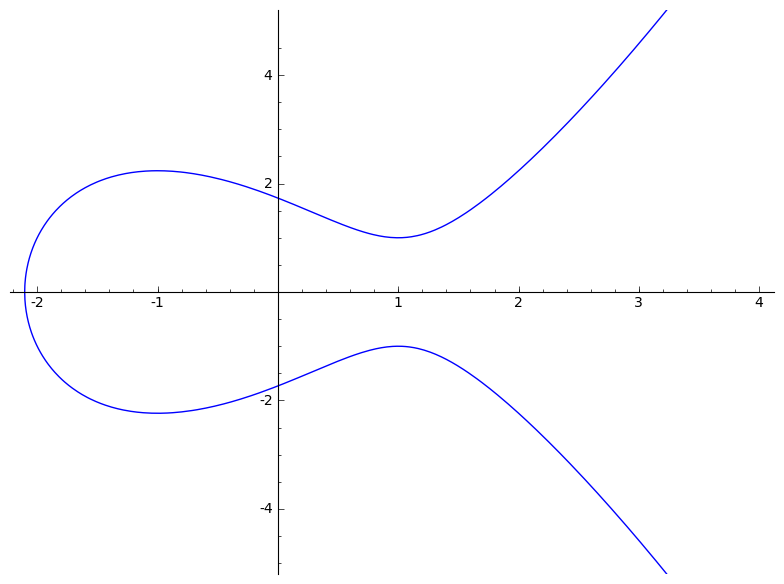
\includegraphics[scale=0.30]{figures/wc1.png}}
        \qquad\qquad
        \subfigure[$y^2 = x^3 - 2x$]{
            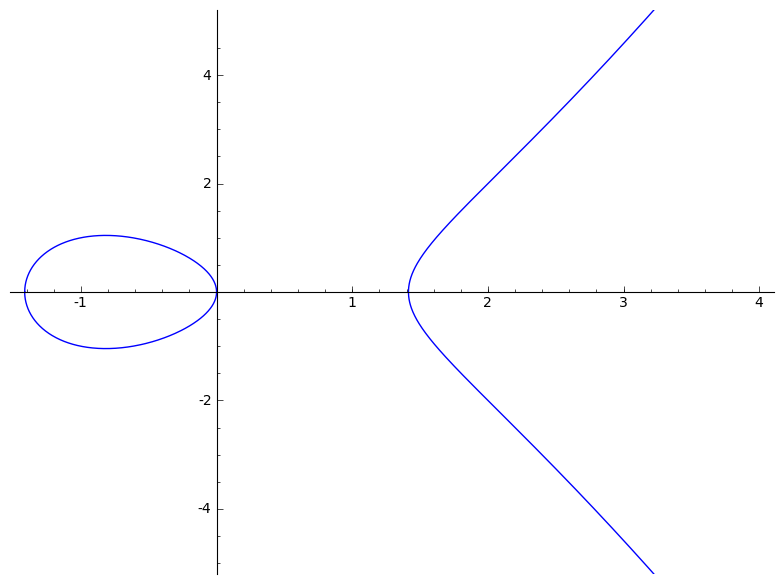
\includegraphics[scale=0.30]{figures/wc2.png}}
    }
    \caption{Two Non-singular Elliptic Curves over $\mathbb{R}$}
    \label{fig:wc1wc2}
\end{figure}

\begin{figure}[htbp]
    \mbox{
        \centering
        \subfigure[$y^2 = x^3$]{
            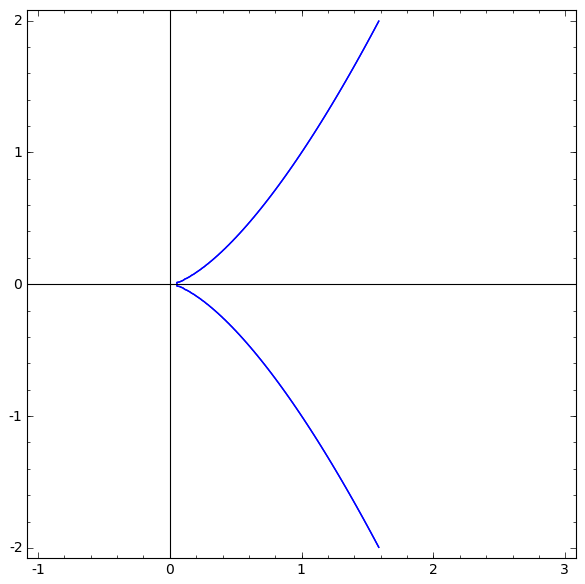
\includegraphics[scale=0.35]{figures/wc3.png}}
        \qquad\qquad
        \subfigure[$y^2 = x^3 + 2x^2$]{
            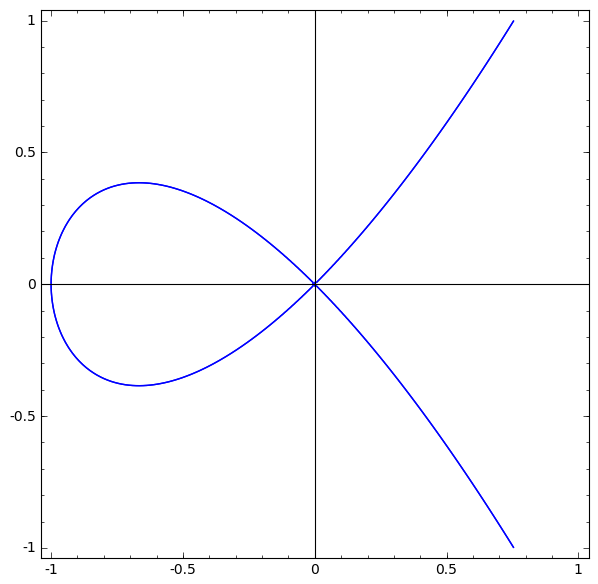
\includegraphics[scale=0.35]{figures/wc4.png}}
    }
    \caption{Two Singular Elliptic Curves over $\mathbb{R}$}
    \label{fig:wc3wc4}
\end{figure}

From here on in, we will use the notation $E(K)$ to specify an elliptic curve
    $E$ over a field $K$, or just $E$ if the field $K$ is understood.
That is,
\[
E(K) = \{\infty\} \cup \{(x, y) \in K \times K \mid 
    y^2 + a_1xy + a_3y^2 = x^3 + a_2x^2 + a_4x + a_6\}
\]
    keeping in mind that we include the ``point at infinity'' $\infty$ among
    the rational points as well.


\bodysubsection{The Group Law}

As it turns out, there's a relatively easy to understand way to define a group
    law on $E(K)$.
In this section, we'll mostly be working with $\mathbb{R}$ as our field for
    ease of notation, understanding, and graphing, but keep in mind that any
    field $K$ works just as well.
Given two points $P$ and $Q$ on $E$ over $\mathbb{R}$ with rational
    coordinates, connect them with a line; that line will (barring a few
    special cases) intersect the graph of $E$ at a third point $R^\prime$ with
    rational coordinates.
Then $R = P + Q$ is defined to be the other point where the vertical line
    through $R^\prime$ intersects the graph of $E$.
In Figure \ref{fig:wgl}, the red line connects $P$ to $Q$ on the curve
    $E: y^2 = x^3 - 3x^2 + 4$.
This line hits the curve at $R^\prime$ in the first quadrant; the green line
    connects this to $P + Q = R$.
\begin{figure}[htbp]
  \centering
  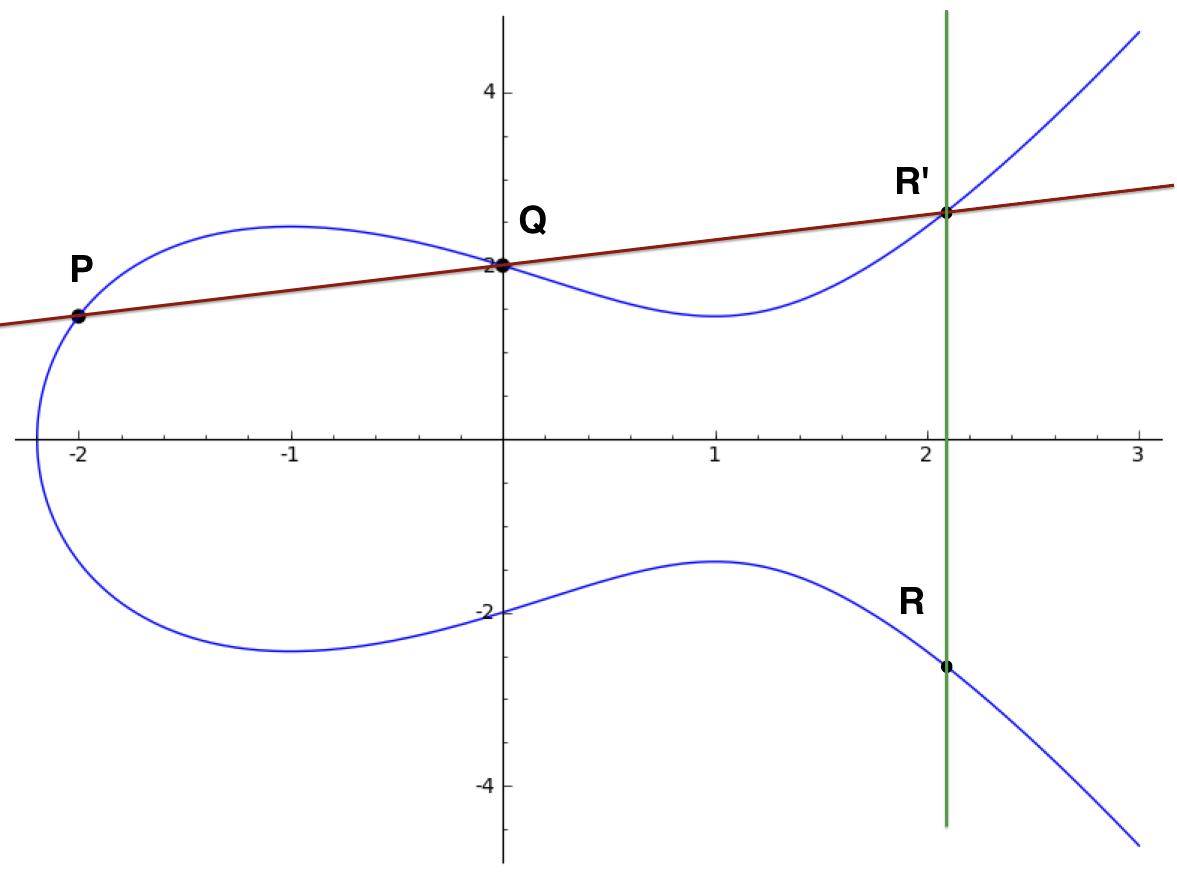
\includegraphics[scale=0.5]{figures/wgl.png}
  \caption{Weierstrass Group Law}
  \label{fig:wgl}
\end{figure}

To go from our ``chord-and-tangent'' geometric understanding to an algebraic
    one, we can use the slope of the red line (via a implicit differentiation
    of $E$'s equation, if necessary) to find $R^\prime$, then the equation of
    the curve to find $R$.
In special cases where the red line is vertical, we either have $P + (-P)
    = \infty$, the point at infinity (the identity element of our group), or $P
    + \infty = P$.
This leads us to the following for curves given in short Weierstrass form:
\begin{thm}[Weierstrass Group Law]\label{thm:wgl}
  The following formulas defining the addition of $P = (x_1,  y_1)$ and $Q =
  (x_2, y_2)$ on $E(\mathbb{R}): y^2 = x^3 + Ax + B$ turns the points
  $E(\mathbb{R})$ into an abelian group:
  \begin{enumerate}
  \item If $P = \infty$, $P + Q = Q$.
  \item If $Q = \infty$, $P + Q = P$
  \item If $x_1 \ne x_2$, $P + Q = (x_3, y_3)$ where
    \begin{displaymath}
      x_3 = m^2 - x_1 - x_2, \qquad y_3 = m(x_1 - x_3) - y_1, \qquad
      \text{ and } m = \frac{y_2 - y_1}{x_2 - x_1}
    \end{displaymath}
  \item If $x_1 = x_2$ but $y_1 \ne y_2$, $P + Q = \infty$
  \item If $P = Q$ and $y_1 \ne 0$, $P + Q = (x_3, y_3)$ where
    \begin{displaymath}
      x_3 = m^2 - 2x_1, \qquad y_3 = m(x_1 - x_3) - y_1, \qquad
      \text{ and } m = \frac{3x_1^2 + A}{2y_1}
    \end{displaymath}
  \item If $P = Q$ and $y_1 = 0$, $P + Q = \infty$
  \end{enumerate}
\end{thm}
The proof of this theorem, though not terribly difficult, is a bit tedious.
As such we will omit it, but it can be found in any text on elliptic curves or
    elliptic curve cryptography, e.g. \cite{washington2008elliptic},
    \cite{silverman2009arithmetic} (section III.2),
    \cite{koblitz2004algebraic}, \cite{cohen2005handbook}, etc.
Again, such a proof would work for any field of characteristic not equal to two
    or three; in those cases, a similar set of formulas can be found.
Of course, in finite fields our geometric understanding doesn't exactly hold
    any more---it is rather difficult to graph in $\mathbb{F}_{8675309}$, for
    example, but the algebraic structure still holds.
Similar theorems work for fields of characteristic $2$ or $3$.
One other thing to note about the above group law is that it involves a number
    of special cases; there isn't a single simple law that holds for any two
    points $P$ and $Q \in E$, and the outcome of $P + Q$ highly depends on the
    relationships between $P, Q,$ and $\infty$.
This will be important to remember when we contrast Weierstrass curves with
    Edwards curves later on.

Over a finite field $K = \mathbb{F}_q$ where $q = p^n$ for some prime $p$ and
    $n \in \mathbb{N}\setminus\{0\}$, similar algebraic work yields an abelian
    group of $\mathbb{F}_q$-rational points on $E$.
This group is very nice to work with; more precisely, we have the following
    (\cite{hankerson2004guide}'s Theorem 3.12):
\begin{thm}[Group Structure of $E(\mathbb{F}_q)$]
Let $E$ be an elliptic curve defined over $\mathbb{F}_q$.
    Then $E(\mathbb{F}_q)$ is isomorphic to the direct sum of cyclic groups
    $\mathbb{Z}_{n_1} \oplus \mathbb{Z}_{n_2}$ for some uniquely determined
    $n_1$ and $n_2 \in \mathbb{N}$ such that $n_2\vert n_1$ and $n_2 \vert
    (q-1)$.
\end{thm}
Since cyclic groups are generated by a single element, the fact that
    $E(\mathbb{F}_q)$ is isomorphic to the direct sum of two cyclic groups (or
    one, if $n_2 = 1$) make them very nice to work with computationally.
The exact details of this isomorphism are rather difficult to specify, however.
Except for specific groups that have thoroughly examined (or worked on via
    Schoof's Algorithm, see \cite{stinson2005cryptography}), the best we can
    easily find are some bounds on $\#E(\mathbb{F}_q)$, the order of the group
    $E(\mathbb{F}_q)$---even though it will of course be $n_1 \cdot
    n_2$---given by the following theorem from the 1930s:
\begin{thm}[Hasse's Theorem]
  The order of the group $E(\mathbb{F}_q)$ satisfies the inequality
  \begin{displaymath}
    q + 1 - 2\sqrt{q} \le \#E(\mathbb{F}_q) \le q + 1 + 2\sqrt{q}
  \end{displaymath}
\end{thm}

In some respects, the fact that the isomorphism $E(\mathbb{F}_q) \to
    C_{n_1} \oplus C_{n_2}$ isn't completely ironed out can seem frustrating.
However, this---along with some other aspects to be discussed shortly---is
    exactly what makes them suitable candidates for cryptographic primitives.


\bodysection{Elliptic Curve Cryptography}

In two groundbreaking papers (\cite{koblitz1987elliptic} and
    \cite{miller1986use}) Koblitz and Miller independently suggested using
    the group of rational points on an elliptic curve as the basis for a public
    key cryptosystem.
In its simplest form, elliptic curve cryptography uses the \textit{Discrete
    Logarithm Problem} and the \textit{Diffie-Hellman Problem} to hide private
    information in public.
We'll give two descriptions of the discrete logarithm problem: one in a
    multiplicative group, like $\mathbb{F}_p^\ast$, and one in an additive one
    like $E(\mathbb{F}_q)$:
\begin{prob}[DLP in multiplicative group]
Given a group $(G, \cdot)$, an element $\alpha \in G$ of order $n$, and an
  element $\beta \in \langle \alpha \rangle$, find the unique element $k \in
  \mathbb{Z}_n$ such that $\alpha^k = \beta$.
\end{prob}
\noindent We'll borrow \cite{stinson2005cryptography}'s notation and say that
    $k = \log_\alpha \beta$.

\begin{prob}[DLP in additive group]
Given a group $(G, +)$, an element $\alpha \in G$ of order $n$, and an element
  $\beta \in \langle \alpha \rangle$, find the unique element $k \in
  \mathbb{Z}_n$ such that $k\alpha = \beta$.
  \end{prob}

As \cite{stinson2005cryptography} says, ``The utility of the Discrete Logarithm
    problem in a cryptographic setting is that finding discrete logarithms is
    (probably) difficult, but the inverse operation of exponentiation can be
    computed efficiently.''
While this description favors multiplicative groups, the idea is the same in an
    additive one: repeated applications of the group operation are (relatively)
    simple to compute, but taking the result of such a computation and trying
    to find the input that yields it is (believed to be) rather difficult.
We'll say more on the ``believed to be'' qualification shortly.

ElGamal cryptosystems are based on the apparent difficulty of the following
problem, first proposed in \cite{diffie1976new}:
\begin{prob}[DHP in multiplicative group]
Given a group $(G, \cdot)$, an element $\alpha \in G$ of order $n$, and two
  elements $\beta = \alpha^b$ and $\gamma = \alpha^c$ in $\langle \alpha
  \rangle$ for some integers $b, c \in \mathbb{Z}_n$, find $\delta =
  \alpha^{bc}$.
\end{prob}
\begin{prob}[DHP in additive group]
Given a group $(G, +)$, an element $\alpha \in G$ of order $n$, and two
  elements $\beta = b \alpha$ and $\gamma = c \alpha$ in $\langle \alpha
  \rangle$ for some $b, c \in \mathbb{Z}_n$, find $\delta = (bc)\alpha$.

\end{prob}
It's apparent that should one find a fast algorithm to compute discrete logs,
    the Diffie-Hellman Problem will also be rather simple to find---once
    $\log_\alpha \beta$ and $\log_\alpha \gamma$ are found, $\delta$ can be
    computed from these two values, since
\[
\delta = \alpha^{bc} = \alpha^{(\log_\alpha \beta)(\log_\alpha \gamma)}
\]
    in multiplicative notation, or
\[
\delta = (bc)\alpha = [(\log_\alpha \beta)(\log_\alpha \gamma)]\alpha
\]
    in additive notation.
Hence the DHP is no harder than the DLP; in many groups, it is believed to be
    as difficult.

The above exposition of the Diffie-Hellman problem is also called the
    \textit{Computational Diffie-Hellman Problem}, to contrast it with the
    \textit{Decisional Diffie-Hellman Problem}:
\begin{prob}[DDHP in additive group]
Given a triple $(\beta, \gamma, \delta)$ from a group $(G, +)$ of order $n$
    such that $\beta = b \alpha$ and $\gamma = c \alpha$ for some $b, c$ chosen
    independently at random from $\mathbb{Z}_n$, determine which of the
    following two cases hold:
\begin{enumerate}
\item   $\delta = (bc)\alpha$
\item   $\delta = d\alpha$ for some other $d$ chosen at random from
    $\mathbb{Z}_n$ independently from $b$ and $c$.
\end{enumerate}
\end{prob}
This problem seems easier to solve at first blush than its computational
    counterpart, but is still rather difficult in many settings.
We rely upon the difficulty of this problem to construct a cryptosystem in
    Chapter \ref{chp:app}.

We now describe how these problems are used for the ElGamal public key
    cryptosystem in $\mathbb{F}_p^\ast$ using two favorite characters from
    cryptographic literature: Alice and Bob.\footnote{The following exposition
    is Cryptosystem 6.1 from \cite{stinson2005cryptography}.}

\begin{cryp}[ElGamal over $\mathbb{F}_p^\ast$]
Suppose Alice wishes to set up a secure way for Bob to send her a message.
They first agree on a large prime $p$ and a group element $\alpha \in
    \mathbb{F}_p^\ast$ that is a generator of the cyclic subgroup of quadratic
    residues (i.e. the set of $\gamma$ for which $\exists \beta \in
    \mathbb{F}_p^\ast$ such that $\beta^2 = \gamma$; this requirement is
    conjectured to equate the semantic security of the
    cryptosystem to solving the DLP).
Next, Alice chooses an integer $a$ (reduced modulo the order of $\alpha$) as
    her secret key and publishes $\alpha$ and $\beta = \alpha^a$.

To send a message (that's been encoded as an integer $m < p$ in some public
    fashion) securely to Alice, Bob chooses a secret integer $b$, computes
\[
(\gamma, \delta) = (\alpha^b, m\beta^b)
\]
    and transmits them to Alice.

Once she has the pair $(\gamma, \delta)$, Alice computes
\[
\delta(\gamma^a)^{-1}
    =   (m\beta^b)(\alpha^{ab})^{-1}
    =   m\alpha^{ab}\alpha^{-ab}
    =   m
\]
    and recovers the message.
\end{cryp}

The security of this system, as mentioned above, is conjectured to be
    equivalent to the feasibility of solving the discrete logarithm problem in
    this group.
That is, this system is secure as long as computing $a$ from $\alpha$ and
    $\beta$ is difficult.
To achieve this, \cite{stinson2005cryptography} states that because of rather
    efficient methods (subexponential time, but not polynomial time) for
    computing $\log_\alpha \beta$ in $\mathbb{F}_p^\ast$ like the index
    calculus algorithm, ``$p$ needs to be at least $2^{1880}$'' for this system
    to securely hide message until the year 2020.\footnote{
        \cite{stinson2005cryptography} was published in 2005.}
As we'll see, the DLP is currently much more secure in $E(\mathbb{F}_q)$ for
    much smaller key sizes.

In elliptic curve cryptography, the size of our finite field $q = p^n$ for some
    prime $p$, the details of the curve $E$, and a special point $P$ are chosen
    in a manner such that the order of $P$ is a prime equal to $\sfrac{\#E}{h}$
    for some small cofactor $h = 1, 2,$ or $4$.
Typically $q = p$ (so $n = 1$) if $p$ is a large odd prime, while $n$ is chosen
    large in the binary case where $p = 2$; see \cite{gallagher09fipspub} for
    more details.
As above, Alice chooses a secret $a$ (reduced modulo $P$'s order) and publishes
    both $P$ and $Q = aP$.

However, implementers of elliptic curve cryptography are currently able to
    choose much smaller parameters than there counterparts in other settings,
    as \cite{stinson2005cryptography} explains:
\begin{quote}
In order for an elliptic curve discrete logarithm based cryptosystem to be
    secure until the year 2020, it has been suggested that one should take $p
    \approx 2^{160}$ [if $p$ is odd] (or $n \approx 160$ [if $p = 2$]).
In contrast, $p$ needs to be at least $2^{1880}$ [in the $F_p^\ast$ case] to
  achieve the same (predicted) level of security.
The reason for this significant difference is the lack of a known index
    calculus attack on elliptic curve discrete logarithms.
\end{quote}
Because the faster DLP algorithms in $\mathbb{F}_p^\ast$ are too specialized to
    work in $E(\mathbb{F}_q)$, would-be attackers are (currently) forced to use
    more generalized algorithms that are much slower, viz. exponential in the
    bit-length of our parameters.
The following table from \cite{agency2009lr} describes the state of affairs as
of 2009:
\begin{table}[htbp]
  \centering
  \begin{tabular}[htbp]{| c | c | c |}
    \hline
    Symmetric Key & RSA \& Diffie-Hellman Key & Elliptic Curve Key\\
    \hline
    80 & 1024 & 160\\
    112 & 2048 & 224\\
    128 & 3072 & 256\\
    192 & 7680 & 384\\
    256 & 15360 & 521\\
    \hline
  \end{tabular}
  \caption{NIST recommended key sizes (measured in number of bits)}
  \label{tab:nrks}
\end{table}

As you can see from table (\ref{tab:nrks}), elliptic curves provide a strong
    alternative to other primitives for public key cryptosystems.
They can make use of this speed and ease of implementation in the following
    cryptosystem to securely share a session key for, say, a communication via
    a faster symmetric system like AES \cite{daemen2002design}:
\begin{cryp}[Diffie-Hellman Key Exchange]
Suppose Alice and Bob wish to construct a secret key with which they can
    communicate privately.
To start, they select a finite field $\mathbb{F}_q$ and a curve
    $E: y^2 = x^3 + Ax + B \bmod p$ (again, $p > 3$).
They also agree on a generator $P$ of a large subgroup $\langle P \rangle$ of
    $E(\mathbb{F}_q)$.

On her own, Alice selects a secret random element $a \in \mathbb{F}_q$ and
    computes $aP = (x_a, y_a)$ and sends it to Bob over an unsecured channel.
Likewise, Bob picks a secret $b$ and computes $bP = (x_b, y_b)$ and sends it to
    Alice.
Then, since $a(bP) = b(aP)$, they now have a shared secret key with which to
    communicate.

Moreover, an eavesdropper (Eve, say) would need either $a$ or $b$ to be able to
    recover their shared key.
However, all Eve can see is $aP$ and $bP$, so she'd need to compute a discrete
    logarithm to recover $a$ or $b$ from these multiples of $P$.
If instead she hopes to compute $abP$ from $aP$ and $bP$, she needs to solve
    the Diffie-Hellman problem, which is also believed to be quite difficult.
\end{cryp}

We conclude this section with an example of using elliptic curves for a
    Diffie-Hellman key exchange.
Computations in this section were done with the help of the Sage computer
    algebra system \cite{sage}.

\begin{ex}
To start, they follow \cite{gallagher09fipspub}'s recommendations and select
    their finite field to be $\mathbb{F}_p$ where
\[
p =  6277101735386680763835789423207666416083908700390324961279
\]
    is a prime of bit length 192.
They then pick their curve $E$ to be $y^2 = x^3 - 3x + B \bmod p$, where
\[
B = 2455155546008943817740293915197451784769108058161191238065
\]
Then per \cite{gallagher09fipspub} their generator $P$ is the point $(x, y)$,
    where
\begin{align*}
x &= 602046282375688656758213480587526111916698976636884684818\\
y &= 174050332293622031404857552280219410364023488927386650641
\end{align*}
Alice selects her secret random element $a \in \mathbb{F}_p$ to be
\[
a = 5599623221253947648338288897360753975761411887111443672469
\]
She then computes $a P = (x_a, y_a)$ where
\begin{align*}
x_a &= 5920503522293796254308104329764746582035708243035924352637\\
y_a &= 4916733057056312203451479844149885752636863324862895552670
\end{align*}
    and sends it to Bob (over an unsecured channel).
Likewise, Bob selects the secret random $b \in \mathbb{F}_p$ where
\[
b = 2188359882031140101779611982450016865481691553092225796933
\]
    and sends $b P = (x_b, y_b)$ to Alice, where
\begin{align*}
x_b &= 763794420572335512449180732023082145057259616577775194615\\
y_b &= 679692871035831936640161559745188598378636802338357105905
\end{align*}
Their shared key is now
\begin{align*}
x   &=  1714835006422896682007668925679643931430048350714705849982\\
y   &=  4464950417588212505755764847617981239405229107427517838554
\end{align*}

Here's the transcript of a \texttt{Sage} session for this
    computation:\footnote{Note that the calls to \texttt{K.random\_element()}
    will in all likelihood yield different values for $a$ and $b$ than those
    given above.}
\lstinputlisting[caption={Diffie-Hellman Example},language=Python]{listings/dh.sage}
The hexadecimal strings for $B$, $x$, and $y$, along with the choice of $p$,
    are all given in \cite{gallagher09fipspub}.
\end{ex}

\bodysection{Edwards Curves}

Inspired by studying the work of Euler and Gauss, Edwards found a new normal
    form of elliptic curves in his 2007 paper \cite{edwards2007normal}.
``In notes published posthumously in his \textit{Werke},'' writes Edwards,
    ``Gauss stated explicitly the formulas Euler had hinted at earlier'' for an
    explicit addition formula on the curve $x^2 = y^2 + x^2y^2 = 1$ which
    related to the integral 
\[
\int \frac{dx}{\sqrt{1 - x^4}}
\]
    Gauss was studying via the change of coordinates $z = y(1 + x^2)$.
Gauss wrote the formulas as
\[
S = \frac{sc^\prime + s^\prime c}{1 - ss^\prime cc^\prime}
\qquad\qquad
C = \frac{cc^\prime - ss^\prime}{1 + ss^\prime cc^\prime}
\]
As Edwards notes in \cite{edwards2007normal}, ``Gauss's choice of the letters
    $s$ and $c$ brings out the analogy with the addition laws for sines and
    cosines.''
Edwards generalized these laws to the curve
\begin{equation}
\label{eq:Ed1}
x^2 + y^2 = a^2 + a^2x^2y^2
\end{equation}
    over a field $K$ where $a \in K$ is a constant such that $a^5 \ne a$.
An example of a curve of this type is given in Figure \ref{fig:ec1}.
\begin{figure}[htbp]
  \centering
  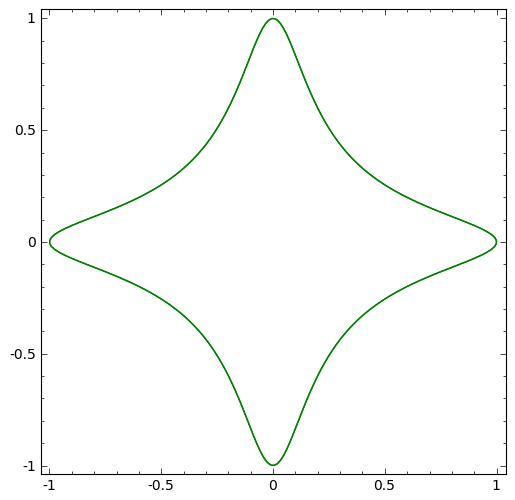
\includegraphics[scale=0.5]{figures/ec1.png}
  \caption{Edwards Curve}
  \label{fig:ec1}
\end{figure}

For the curve in equation \ref{eq:Ed1}, we have the following group law:
\begin{thm}(Edwards Addition Law)
If $a$ is a constant for which $a^5 \ne a$, the formulas
\[
X = \frac{1}{a} \cdot \frac{xy^\prime + yx^\prime}{1 + xyx^\prime y^\prime}
\qquad\qquad
Y = \frac{1}{a} \cdot \frac{yy^\prime - xx^\prime}{1 - xyx^\prime y^\prime}
\]
    describe the addition formula for the elliptic curve 
\[
x^2 + y^2 = a^2 + a^2x^2y^2
\]
\end{thm}
This is theorem (3.1) in \cite{edwards2007normal}; the reader is referred there
    for a proof.
By simple inspection, one can see that the neutral element for this curve is
    $(0, a)$.
Moreover, the inverse $-P$ of the point $P = (x, y)$ is $(-x, y)$:
\begin{align*}
(x, y ) + (-x, y)
    &=  \left( \frac{1}{a} \cdot \frac{xy - yx}{1 - x^2y^2},
               \frac{1}{a} \cdot \frac{y^2 + x^2}{1 + x^2y^2} \right)\\
    &=  \left(0, \frac{1}{a} \cdot \frac{a^2 + a^2x^2y^2}{1 + x^2y^2} \right)\\
    &=  (0, a)
\end{align*}
    using the curve equation in the intermediate step.

As Edwards points out in his proposition (5.1), every curve of the form given
    in equation \ref{eq:Ed1} is \textit{birationally equivalent} to an
    elliptic curve in Weierstrass form.
That is, following Edwards' advice ``to abandon the notion of \textit{points
    of} a curve and to work instead with \textit{rational functions of} a
    curve, one can consider two curves birationally equivalent ``if their
    fields of rational functions are isomorphic.''
We'll discuss this idea in more depth when we go into the details of Bernstein
    and Lange's exploration of Edwards curves.

The addition law given in the above theorem is much simpler than the equivalent
    Weierstrass one given in an earlier section.
There are no special cases, no changing the rules depending on whether $P$ is
    the identity element or $P = -Q$.
We do of course lose the simple geometric description of Weierstrass
    curves\footnote{Though as we'll see in Chapter \ref{chp:pair}, there is
    another geometric interpretation of the group law here.}, but
    that is a small price to pay for so simple, symmetric, and elegant a group
    law.
As we'll see in the next section, the Edwards curve group law's superiority is
    more than just aesthetic: it has desirable consequences for elliptic curve
    cryptographic schemes that use Edwards curves as their group.


\bodysection{Bernstein \& Lange: ECC potential}

In \cite{bernstein2007faster}, Bernstein and Lange generalize Edwards' original
    curve to more cases and turn their attention to cryptographic viability.
First, though, we explain the necessary algebraic geometry.

\bodysubsection{Algebraic Geometry}

Strictly speaking, a curve is ``a projective variety of genus one'' and
    dimension one with a distinguished rational point
    (\cite{silverman2009arithmetic}), so working more in depth with elliptic
    curves requires some understanding of algebraic geometry.
We give a cursory sketch of the necessary pieces based upon
    \cite{silverman2009arithmetic} and \cite{hartshorne1977algebraic}; readers
    who wish for more in-depth coverage of these topics are referred to these
    texts.

First off, in many cases it makes sense to work with projective coordinates (as
    mentioned above) instead of affine ones.
As we saw in the case of Weierstrass curves, sometimes this is not just for
    convenience; we need projective coordinates to be able to discuss the point
    at infinity that arises from adding two points with the same
    $x$-coordinate, for example.
\begin{dfn}
\textit{Projective $n$-space} over a field $K$, denoted by $\mathbb{P}^n(K)$ or
    just $\mathbb{P}^n$, is the set of all $n + 1$ tuples in regular affine
    coordinates
\[
(X_0 , \ldots, X_n) \in \mathbb{A}^{n + 1}
\]
    such that at least one $X_i$ is nonzero, together with the following
    equivalence relation:
\[
(X_0 , \ldots, X_n) \sim (Y_0, \ldots, Y_n)
\]
    if $\exists \lambda \in \overline{K}^\ast$ such that $X_i = \lambda Y_i$
    for each $i$.
We denote an equivalence class by $(X_0 : \ldots: X_n)$, and the individual
    $X_i$ are called \textit{homogeneous} coordinates.
\end{dfn}

Next up is the concept of a \textit{variety}.
Though \cite{silverman2009arithmetic} and \cite{hartshorne1977algebraic}
    subscribe to stricter (or at least more precise) definitions, for our
    purposes the ideas from \cite{adams1994introduction} will suffice.
\begin{dfn}
Given a polynomial $f$ from $\mathbb{P}^n(K)$ to $K$, the \textit{variety}
    $V(f)$ is the set of solutions of the equation $f = 0$.
More formally,
\[
V(f) = \{(X_0 : \ldots: X_n) \in \mathbb{P}^n \mid f(X_0 : \ldots X_n) = 0\}
\]
\end{dfn}

Next we define rational maps between varieties.
\begin{dfn}
Let $V_1, V_2 \subset \mathbb{P}^n$ be projective varieties.
A \textit{rational map} from $V_1$ to $V_2$ is a map of the form
\[
\varphi: V_1 \to V_2, \varphi = (f_0 : \ldots: f_n)
\]
    where the $f_i$ have the property that for every point $P \in V_1$ for
    which all of $f_0,\ldots,f_n$ are defined,
\[
\varphi(P) = (f_0(P): \ldots:f_n(P)) \in V_2
\]
\end{dfn}
Note that a rational map $\varphi: V_1 \to V_2$ need not be a well-defined
    function at every point in $V_1$; however, it may be possible to replace
    each $f_i$ with $gf_i$ for some other rational function $g$ to evaluate
    $\varphi$ at a troublesome point $P \in V_1$.

Finally, we come to birational maps.
\begin{dfn}
A \textit{birational map} is a rational map that admits an inverse; i.e. a
    rational map $\varphi: V_1 \to V_2$ for which there is another rational map
    $\psi: V_2 \to V_1$ such that, when defined, $\varphi \circ \psi$ and $\psi
    \circ \varphi$ are the identity map.
If there is a birational map from a variety $V_1$ to a variety $V_2$, we say
    that these two varieties are \textit{birationally equivalent}.
\end{dfn}
Birational equivalence gives a looser sort of connection between two varieties
    (or curves, since that's what we are focused on) than strict isomorphism.
Basically, two varieties are birationally equivalent if, except for a handful
    of points, they are isomorphic.
In algebraic geometry, singularities of birational maps are typically handled
    by ``blowing up''\footnote{Think ``blowing up a balloon,'' not ``blowing up
    Wile E. Coyote.''} the maps at those points to resolve them.
If a point $(x_0, y_0)$ is a singularity of a map $\varphi$, we can set $y =
    tx$ for some variable $t$ and evaluate what happens as $y \to y_0$.
We'll show an example of this when we discuss binary Edwards curves in Chapter
    \ref{chp:bec}; for more, see a text on algebraic geometry like
    \cite{hartshorne1977algebraic}.


\bodysubsection{Bernstein \& Lange's Edwards Curves}

As the authors mention in the start of \cite{bernstein2007faster}, ``Every
    elliptic curve over a non-binary field is birationally equivalent to a
    curve in Edwards form over an extension of the field, and in many cases
    over the original field.''
Because ``every Edwards curve has a point of order 4,'' to be birationally
    equivalent to a curve without such a point, such as ``the NIST curves over
    prime fields,'' may require working over an extension field.
However, ``to capture a larger class of elliptic curves over the original
    field,'' Bernstein and Lange generalized the definition of Edwards curves
    to the following:
\begin{dfn}
For a fixed field $K$ of characteristic not equal to two, choose $c, d \in K$
    such that $cd(1 - dc^4) \ne 0$ (so $c \ne 0, d \ne 0,$ and $dc^4 \ne 1$).
The \textit{Edwards elliptic curve} or \textit{Edwards curve} defined by $c$
    and $d$ is the (affine) curve of the form
\begin{equation}\label{eq:bled}
x^2 + y^2 = c^2(1 + dx^2y^2)
\end{equation}
\end{dfn}
This definition covers ``more than $\sfrac{1}{4}$ of all isomorphism classes of
    elliptic curves over a finite field,'' so it is a more useful definition
    for our purposes.
Moreover, they show that these are isomorphic to curves where $c = 1$, we will
    stay with the more general form given in \ref{eq:bled}.
From now on we will use this definition when we talk of Edwards curves.
In order to distinguish it from twisted Edwards curves (next section) and
    binary Edwards curves (next chapter), we'll denote the Edwards curve given
    by equation \ref{eq:bled} by $E_{O,c, d}$.

Per theorem (2.1) in \cite{bernstein2007faster}, $E_{O, c, d}$ is birationally
    equivalent to the Weierstrass curve
\[
\left(\frac{1}{1 - dc^4}\right)v^2
    =   u^3 + 2\left(\frac{1 + dc^4}{1 - dc^4}\right)u^2 + u
\]
    via the birational map
\[
(x, y)  \mapsto (u, v)
    =   \left(\frac{1 + y}{1 - y}, \frac{2(1 + y)}{x(1 - y)}\right)
\]
    (since there are only finitely many points with $x(1 - y) = 0$, this is
    indeed a birational map), with inverse
\[
(u, v)  \mapsto (x, y)
    =   \left(\frac{2u}{v}, \frac{u - 1}{u + 1}\right)
\]
    (again, there are only finitely many points such that $(u + 1)v = 0$).

Like Edwards's original formulation, this curve has a simple, symmetric group
    law.
\begin{thm}[Bernstein \& Lange Edwards Addition Law]
For two points $(x_1, y_1)$ and $(x_2, y_2)$ on the Edwards curve $E_{O, c, d}$
    given by equation \ref{eq:bled}, the map
\[
(x_1, y_1), (x_2, y_2) \mapsto
\left(
    \frac{x_1y_2 + y_1x_2}{c(1 + dx_1x_2y_1y_2)}
    ,
    \frac{y_1y_2 - x_1x_2}{c(1 - dx_1x_2y_1y_2)}
\right)
\]
    turns the set of rational points on $E_{O, c, d}(K)$ into an abelian group.
The neutral element for this group law is $\mathcal{O} = (0, c)$, and the
    inverse of the point $(x, y)$ is $(-x, y)$.
\end{thm}
For a proof of this, see theorems (3.1) and (3.2) in
    \cite{bernstein2007faster}.

Critics may wonder why cryptographic researchers are so interested in another
    normal form for elliptic curves.
At first blush, this new normal form may even seem less useful than the
    familiar Weierstrass form since it requires a point of order four.
As we'll see in the last section of this chapter, however, the benefits of
    Edwards curves far outweigh the drawbacks.
For now, though, we'll briefly touch on one other type of Edwards curves.

\bodysubsection{Twisted Edwards Curves}

For the sake of completeness, we now define twisted Edwards
    curves.\footnote{Since they have been the main focus of research for things
    like pairings over Edwards curves; see Chapter \ref{chp:app}.}

In \cite{bernstein2008twisted}, Bernstein et. al. introduced a generalization
    of Edwards curves dubbed ``twisted Edwards Curves.''
These curves ``include more curves over finite fields,'' including ``every
    elliptic curve in Montgomery form'' (another form garnering cryptographic
    interest).
As \cite{arene2011faster} explains, their name ``comes from the fact that the
    set of twisted Edwards curves is invariant under quadratic
    twists\footnote{A \textit{quadratic twist} of a curve is another curve
    isomorphic to it over a field extension of degree two.} while a quadratic
    twist of an Edwards curve is not necessarily an Edwards curve.''

\begin{dfn}
For a field $K$ with $char(K) \ne 2$, and distinct nonzero elements $a, d \in
    K$, the \textit{twisted Edwards curve} $E_{T, a, d}(K)$ is the curve
\[
ax^2 + y^2 = 1 + dx^2y^2
\]
\end{dfn}

As you can see, if $a = 1$, then $E_{T, a, d}$ is an Edwards curve with $c =
    1$.
Furthermore, $E_{T, a, d}$ is a quadratic twist of the Edwards curve $E_{O, 1,
    \sfrac{d}{a}}$
\[
\overline{x}^2 + \overline{y}^2
    =   1 + (\sfrac{d}{a})\overline{x}^2\overline{y}^2
\]
    via the map
\[
(\overline{x}, \overline{y}) \mapsto (x, y)
    =   (\sfrac{\overline{x}}{\sqrt{a}}, \overline{y})
\]
    over the field extension $K(\sqrt{a})$.
Of course, if $a$ is a square in $K$ then these curves are isomorphic over $K$
    itself.

As before, this curve also has a symmetric and elegant group law.
\begin{thm}[Twisted Edwards Addition Law]
Let $(x_1, y_1), (x_2, y_2)$ be two points on the twisted Edwards curve
    $E_{T, a, d}$ given by $ax^2 + y^2 = 1 + dx^2y^2$.
Then the map
\[
(x_1, y_1), (x_2, y_2) \mapsto
\left(
    \frac{x_1y_2 + y_1x_2}{1 + dx_1x_2y_1y_2}
    ,
    \frac{y_1y_2 - ax_1x_2}{1 - dx_1x_2y_1y_2}
\right)
\]
    turns the set of rational points on $E_{T, a, d}(K)$ into an abelian group.
The neutral element for this curve is $(0, 1)$ and the inverse of $(x, y)$ is
    $(-x, y)$.
\end{thm}
For a proof, see \cite{bernstein2008twisted}.

In the next chapter, we'll define binary Edwards curves, a form of elliptic
    curve that is similar in flavor to the above ones except that it is
    defined over fields of characteristic two.
First, though, we'll explain the cryptographic appeal of Edwards curves.

\bodysection{Cryptographic Safety from the Mathematical Foundation}

As one can see from the operation counts given for the explicit formulas for
addition and doubling on Edwards and twisted Edwards curves given in
    \cite{bernstein2007faster} and \cite{bernstein2008twisted}\footnote{Which
    we incorporate into \texttt{e2c2}; see Appendix \ref{chp:src}.}, these new
    curves outperform Weierstrass curves with regards to pure speed.
For abelian groups that form the basis of cryptographic protocols, faster
    computations and more efficiency are certainly very important.
However, binary Edwards curves produce a group law that in pure operation
    counts is a bit slower than its Weierstrass counterpart.\footnote{Slower
    only if we don't take validity checks into account; if we do, per
    \cite{moloneyefficient}, then the binary Edwards group law is still
    competitive.}
As it turns out, the Edwards family of curves is cryptographically interesting
    for a different reason: their groups laws are \textit{unified} and
    \textit{complete}, which leads to implementations that are safer against
    certain types of attacks from the very start; they have greater security
    ``baked into them'' from their mathematical foundation, as it were.

As we mentioned in a previous section, elliptic curve cryptography offers a lot
    of security for relatively low cost because of the lack of subexponential
    algorithms for calculating discrete logarithms.
As such, attackers trying to break ECC implementations tend to focus on the
    technical details of a specific implementation rather than any mathematical
    or algorithmic attacks which may take too long.
Indeed, ``the mathematically proved security of a cryptosystem does not imply
    its implementation [has] security against side-channel attacks,'' as
    \cite{reddy2009elliptic} explains.
A side-channel attack on a cryptosystem implementation is one that attempts to
    gain secret information via measuring some aspect of the implementation's
    performance that, perhaps unknown to its designers or users, leaks such
    information.
Examples for ECC implementations include ``those that monitor the power
    consumption and/or the electromagnetic emanations of a device,''
    \cite{reddy2009elliptic} expands, ``and can infer important information
    about the instructions being executed or the operands being manipulated at
    a specific instant of interest.''
Elliptic curve cryptography with Weierstrass curves is certainly quite
    vulnerable to such attacks;\footnote{At least in the ``textbook'' version
    we've presented, of course.}
The group law as presented in theorem \ref{thm:wgl} has a number of special
    cases one must check for; any implementation needs to check whether either
    of the points it's trying to add is $\infty$, if the two points have the
    same $x$-coordinate but are different points, if they are the same but have
    an $x$-coordinate of zero (so they lie on the same vertical line), or if
    the two points are equal and have a nonzero $x$-coordinate.

There are a multitude of papers detailing such attacks against ECC or trying to
    safeguard systems against them; see \cite{billet2003jacobi,
    brier2002weierstrass, brumley2011timing, chevallier2004low,
    coron1999resistance, goubin2002refined, izu2002exceptional,
    izu2002improved, joye2003elliptic, joye2001hessian, moller2001securing},
    and \cite{okeya2000power} just to name a few.
With all that energy expended on attacking elliptic curve cryptosystems from
    the implementation side, it would certainly be advantageous for a system to
    have a group law that protects against such attacks from the start; this is
    where Edwards curves come in.

As \cite{bernstein2007faster} proves, the group law for an Edwards curve $E_{O,
    c, d}$ is \textit{unified}, since it can also be used to double a point.
That eliminates any need to check whether $P = Q$ when trying to add $P + Q$.
Moreover, this same law works for the neutral element and for inverses; this
    eliminates even more special cases.
Finally, if $d$ isn't a square in $K$ then the addition law is
    \textit{complete}; i.e. it works for all pairs of inputs, and there are no
    special cases to check for at all.
Twisted Edwards curves also share the same cryptographic benefits---the group
    law works for doubling, so it is unified, and is complete if $a$ and $d$
    are both nonsquares in $K$ (i.e. $\sqrt{a}, \sqrt{d} \not\in K$).
To reiterate, this strengthens ECC implementations based on these types of
    curves against side-channel analysis and attacks from the start; the
    elegance of their mathematical theory leads to safer, more easily
    implemented cryptography.
As we'll see in the next chapter, binary Edwards curves also have these
    desirable properties.

\bodychapter{Binary Edwards Curves}
\label{chp:bec}

In this chapter we discuss binary Edwards curves.
We'll start with a discussion of the work of \cite{bernstein2008binary}, the
    first paper to lay out an ``Edwards-like'' elliptic curve over a field of
    characteristic two.
Then, we'll look at the practical improvements provided by
    \cite{moloneyefficient}.

Bernstein, Lange, and Farashahi's paper \cite{bernstein2008binary} presented
    ``the first complete addition formulas for binary elliptic curves.''
As such, it was a huge milestone in the field; binary elliptic curves are very
    attractive from an implementation standpoint because, after all, computers
    work in binary.
Until this paper came along, ECC implementations over a binary finite field
    were inherently vulnerable to the types of side-channel attacks mentioned
    in the previous chapter.
Moloney, O'Mahony, and Laurent's paper \cite{moloneyefficient} extended this
    work, presenting algorithms and practical measurements of things like code
    complexity that matter to implementors of cryptographic primitives.

\bodysection{Bernstein, Lange, \& Farashahi}

Unfortunately for cryptographers, the Edwards curve equation $x^2 + y^2 = c^2(1
    + dx^2y^2)$ is not elliptic over fields with characteristic two; if it
    were, one could just use Edwards curves (or twisted Edwards curves) over
    these fields and reap the same benefits that we did over non-binary fields.
In 2008, Bernstein, Lange, and Farashahi came up with a normal form for
    elliptic curves over binary fields that is reminiscent of Edwards curves
    which they dubbed \textit{binary Edwards curves}.

\begin{dfn}
Let $K$ be a field with $char(K) = 2$, and $d_1, d_2 \in K$ such that
    $d_1 \ne 0$ and $d_2 \ne d_1^2 + d_1$.
The \textit{binary Edwards curve} $E_{B, d_1, d_2}$ is the affine curve
\[
d_1(x + y) + d_2(x^2 + y^2) = xy(x + 1)(y + 1)
\]
\end{dfn}

As you can see from the definition, $E_{B, d_1, d_2}$ is symmetric in $x$ and
    $y$, so if $(x, y)$ is a point on $E_{B, d_1, d_2}$ then so is $(y, x)$;
    this will soon yield our negation law.
There are only two points on the curve that are invariant under this law: $(0,
    0)$ and $(1, 1)$.
As we'll see shortly, the former will be our neutral element, while the latter
    will be a point of order two.

In their theorem (2.2), the authors of \cite{bernstein2008binary} show that
    the affine form of $E_{B, d_1, d_2}$ is nonsingular.
Shortly after, they look at singularities of the projective closure
\[
d_1(X + Y)Z^3 + d_2(X^2 + Y^2)Z^2 = XY(X + Z)(Y + Z)
\]
    of which there are two: $\Omega_1 = (1 : 0 : 0)$ and $\Omega_2 = (0 : 1 :
    0)$.
We'll expand on their work to show that the first of these blows up to two
    projective points, and use their same appeal to symmetry to cover the
    second.

To study $E_{B, d_1, d_2}$ around $\Omega_1$, consider the affine curve
    $E_{\Omega_1}$:
\[
d_1(1 + y)z^3 + d_2(1 + y^2)z^2 + y(1 + z)(y + z) = 0
\]
If we take the partial derivatives of this curve with respect to $y$ and $z$,
    we get
\begin{align*}
\frac{\partial E_{\Omega_1}}{\partial y}
    &=  d_1z^3 + 2d_2yz^2 + (z + 1)(y + z) + (z + 1)y\\
    &=  d_1z^3 + 2d_2yz^2 + 2yz + z^2 + 2y + z\\
    &=  d_1z^3 + z^2 + z
\end{align*}
    and
\begin{align*}
\frac{\partial E_{\Omega_1}}{\partial z}
    &=  3(y + 1)d_1z^2 + 2(y^2 + 1)d_2z + (z + 1)y + (y + z)y\\
    &=  3d_1yz^2 + 2d_2y^2z + 3d_1z^2 + 2d_2z + y^2 + 2yz + y\\
    &=  d_1(1 + y)z^2 + y^2 + y
\end{align*}
Evaluating these at the point $(y, z) = (0, 0)$, we see that $E_{\Omega_1}$ is
    indeed singular; we can ``blow up'' this singularity by substituting $y =
    tz$ into $E_{\Omega_1}$ and dividing through by $z^2$, getting the
    following curve $E_t$:
\[
d_1(1 + tz)z + d_2(1 + t^2z^2) + t(1 + t)(1 + z) = 0
\]
If we substitute in $z = 0$, $E_t$ becomes $t^2 + t + d_2 = 0$ which has two
    distinct roots in $\overline{K}$.
To see that these two points are nonsingular, consider the partial derivatives
\begin{align*}
\frac{\partial E_t}{\partial t}
    &=  2d_2tz^2 + d_1z^2 + (z + 1)(t + 1) + (z + 1)t\\
    &=  2d_2tz^2 + d_1z^2 + 2tz + 2t + z + 1\\
    &=  d_1z^2 + z + 1
\end{align*}
    and
\begin{align*}
\frac{\partial E_t}{\partial z}
    &=  2d_2t^2z + d_1tz + (t + 1)t + (tz + 1)d_1\\
    &=  2d_2t^2z + 2d_1tz + t^2 + d_1 + t\\
    &=  t^2 + d_1 + t
\end{align*}
Neither of these partial derivatives vanish at the point $(z, t) = (0, 0)$, so
    these blowups are nonsingular.
As \cite{bernstein2008binary} says, they are ``defined over the smallest
    extension of $K$ in which $d_2 + t + t^2 = 0$ has roots.''

The authors provide the following birational equivalence: the map
\begin{align*}
(x, y)
    &\mapsto    (u, v)\\
    &=  \left(
            \frac{d_1(d_1^2 + d_1 + d_2)(x + y)}{xy + d_1(x + y)}
            ,
            d_1(d_1^2 + d_1 + d_2)\left[
                \frac{x}{xy + d_1(x + y)} + d_1 + 1
            \right]
        \right)
\end{align*}
    is a birational equivalence\footnote{Though we'll use the equivalence given
    in \cite{moloneyefficient} ourselves.} between $E_{B, d_1, d_2}$ and the
    binary elliptic curve $W$\footnote{In shorter Weierstrass form for binary
    curves}
\[
v^2 + uv = u^3 + (d_1^2 + d_2)u^2 + d_1^4(d_1^4 + d_1^2 + d_2^2)
\]
This map has inverse
\[
(u, v) \mapsto (x, y)
    =   \left(
            \frac{d_1(u + d_1^2 + d_1 + d_2)}
                {u + v + (d_1^2 + d_1)(d_1^2 + d_1 + d_2)}
            ,
            \frac{d_1(u + d_1^2 + d_1 + d_2)}
                {v + (d_1^2 + d_1)(d_1^2 + d_1 + d_2)}
        \right)
\]
This map is undefined at the point $(0, 0)$; if we define $(0, 0) \mapsto
    \infty$, then this becomes an isomorphism between the curves.

The addition law on a binary Edwards curve is just as symmetric as its ordinary
    and twisted counterparts, if a little more complicated:

\begin{thm}[Binary Edwards Addition Law]
If $(x_1, y_1)$ and $(x_2, y_2)$ are two points on the binary Edwards curve
    $E_{B, d_1, d_2}$, then the mapping $(x_1, y_1), (x_2, y_2) \mapsto (x_3,
    y_3)$ turns the rational points on this curve into an abelian group, where
\begin{align*}
x_3 &=  \frac{d_1(x_1 + x_2) + d_2(x_1 + y_1)(x_2 + y_2) + (x_1 + x_1^2)
            (x_2(y_1 + y_2 + 1) + y_1y_2)}{d_1 + (x_1 + x_1^2)(x_2 + y_2)}\\
y_3 &=  \frac{d_1(y_1 + y_2) + d_2(x_1 + y_1)(x_2 + y_2) + (y_1 + y_1^2)
            (y_2(x_1 + x_2 + 1) + x_1x_2)}{d_1 + (y_1 + y_1^2)(x_2 + y_2)}
\end{align*}
    as long as the denominators in the above fractions are nonzero.
\end{thm}
Substituting $(0, 0)$ for either $(x_1, y_1)$ or $(x_2, y_2)$ in the above law,
    we see that $(0, 0)$ is the neutral element.
Moreover, $(x, y) + (y, x) = (0, 0)$, so the inverse of a point $(x, y)$ is
    $(y, x)$ as we said before.
When defined, this addition law is unified; it can be used for doubling as
    well.
For a proof of this law, see section 3 of \cite{bernstein2008binary}; in that
    section, the authors demonstrate that this addition law corresponds to the
    addition law on the equivalent Weierstrass curve, so the birational map is
    indeed a isomorphism.

Astute readers will notice the caveat ``as long as the denominators in the
    above fractions are nonzero'' in the previous theorem.
We could try and list all the cases where those fractions don't exist and piece
    together a group law that takes these special cases into account, like the
    Weierstrass group law does.
However, Bernstein, Lange, and Farashahi offer us another very helpful theorem.

\begin{thm}[Complete Binary Edwards Curves]
Let $K$ be a field with $char(K) = 2$ and $d_1, d_2 \in K$ such that $d_1 \ne
    0$ and no element $t \in K$ satisfies $t^2 + t + d_2 = 0$.
Then the addition law on the binary Edwards curve $E_{B, d_1, d_2}(K)$ is
    complete.
Moreover, every ordinary elliptic curve over the finite field
    $\mathbb{F}_{2^n}$ for $n \ge 3$ is birationally equivalent over
    $\mathbb{F}_{2^n}$ to a complete binary Edwards curve.
\end{thm}
See theorems (4.1) and (4.3) for proofs of these claims.
Since elliptic curve cryptography typically involves finite binary fields of
    degree $n$ at least $160$, the above theorem tells us that we can use a
    binary Edwards curve and reap the benefits of a complete and unified group
    law.

Despite their extremely thorough treatment in \cite{bernstein2008binary},
    Bernstein, Lange, and Farashahi did leave some small room for improvement.
In trying to find an equivalent complete binary Edwards curve for a given
    Weierstrass curve, they left some nondeterminism in finding $d_1$.
Though they could find an appropriate $d_1$ easily enough experimentally, they
    didn't have a  deterministic algorithm for it.

\bodysection{Moloney, O'Mahony, \& Laurent}

In 2010, Moloney, O'Mahony, and Laurent posted \cite{moloneyefficient} online.
In it, they perform a practical, implementation-focused analysis of binary
    Edwards curves, and come up with some very useful results.

First, they offer a modified birational equivalence.
Recall the usual trace function
\[
Tr: \mathbb{F}_{2^n} \to \mathbb{F}_2, \qquad
    \alpha \mapsto \sum_{i = 0}^{n - 1} \alpha^{2^i}
\]
    and define the half-trace function
\[
H: \mathbb{F}_{2^n} \to \mathbb{F}_2, \qquad
    \alpha \mapsto \sum_{i = 0}^{\sfrac{(n - 1)}{2}} \alpha^{2^{2^i}}
\]
    (noting that $n$ must be odd).
If given $a_2$ and $a_6$ for a Weierstrass curve, suppose we found a suitable
    $d_1$; we can then calculate
\[
d_2 = d_1^2 + d_1 + \sfrac{\sqrt{a_6}}{d_1^2}
\]
We will also make use of $b$ which satisfies $b^2 + b = d_1^2 + d_2 + a_2$; it
    can be directly calculated as
\[
b = H(d_1^2 + d_2 + a_2)
\]
The authors show that $(u, v) \mapsto (x, y)$ is another birational equivalence
    from the Weierstrass curve to $E_{B, d_1, d_2}$, where
\begin{align*}
x   &=  \frac{d_1(bu + v + (d_1^2 + d_1)(d_1^2 + d_1 + d_2))}
        {u^2 + d_1u + d_1^2(d_1^2 + d_1 + d_2)}\\
y   &=  \frac{d_1((b + 1)u + v + (d_1^2 + d_1)(d_1^2 + d_1 + d_2))}
        {u^2 + d_1u + d_1^2(d_1^2 + d_1 + d_2)}
\end{align*}
Though there is no difference between this equivalence and the one presented by
    Bernstein et.al., the calculation of this equivalence involves fewer field
    inversions.
Field inversions tend to be very costly to calculate, so the fewer the
    better.\footnote{\texttt{e2c2} uses this birational equivalence.}

Secondly, and perhaps more importantly, the authors present two deterministic
    algorithms to find a suitable $d_1$ given $n \ge 3$, $a_2$, and $a_6$
    determining a Weierstrass curve over the finite field $\mathbb{F}_{2^n}$.
We reproduce the first algorithm here, since that's what is used in our
    software library \texttt{e2c2}.
Precompute $t = Tr(a_2)$, $r = Tr(a_6)$, and $w = x + Tr(x)$ where $x$ is the
    indeterminant used to define our field extension $\mathbb{F}_{2^n}$.
This algorithm ``terminates with guaranteed success in a finite number of
    steps, except in the case $t = r = 0$.''
Fortunately, ``this case does not appear in any of the standards (e.g. NIST) of
    which the authors are aware.''

\begin{Algorithm}
\caption{Moloney, O'Mahony, \& Laurent's first $d_1$ finder}
\label{alg:d1}
\begin{algorithmic}
    \Function{MOLalg1}{$n, p, t, r, a_6, w$}
        \If{$t = 0$ and $r = 1$}
            \State $d_1 \gets 1$
        \Else
            \If{$t = 1$ and $r = 0$}
                \State $d_1 \gets \sqrt[4]{a_6}$
            \Else
                \If{$t = r = 1$ and $a_6 \ne 1$}
                    \If{$Tr(\sfrac{1}{a_6 + 1}) = 1$}
                        \State $d_1 \gets \sqrt{a_6} + \sqrt[4]{a_6}$
                    \Else
                        \State $d_1 \gets \sqrt[4]{a_6} + 1$
                    \EndIf
                \Else
                    \If{$t = 1$ and $a_6 = 1$}
                        \If{$Tr(\sfrac{1}{w}) = 1$}
                            \State $d_1 \gets w$
                        \Else
                            \If{$Tr(\sfrac{1}{(w + 1)}) = 0$}
                                \State $d_1 \gets \sfrac{1}{(w + 1)}$
                            \Else
                                \State $d_1 \gets 1 = \sfrac{1}{(w + 1)}$
                            \EndIf
                        \EndIf
                    \Else
                        \If{$t = r = 0$}
                            \If{$Tr(\sfrac{1}{(a_6 + 1)}) = 0$}
                                \State $d_1 \gets \sqrt[4]{a_6} + 1$
                            \Else
                                \State $i \gets 1$
                                \State $s \gets \sqrt{a_6}$
                                \While{$Tr(a_6^{2^i + 1}) = 0$}
                                    \State $s \gets s^2$
                                    \State $i \gets i + 1$
                                \EndWhile
                                \State $d_1 \gets \sfrac{1}{(s + 1)}$
                            \EndIf
                        \EndIf
                    \EndIf
                \EndIf
            \EndIf
        \EndIf
        \State \Return $d_1$
    \EndFunction
\end{algorithmic}
\end{Algorithm}

Finally, \cite{moloneyefficient} offers some valuable measurements and
    comparisons between implementations of Weierstrass and binary Edwards
    curves.
They note that ``implementing ECC from the textbooks leaves us with incredibly
    complex code,'' while implementations of binary Edwards curves have lower
    complexity.
The symmetric, unified, and complete group law takes a lot of the burden off of
    potential developers and implementors.
More interestingly, despite the larger operation count for the binary Edwards
    addition law, the fact Weierstrass implementations must constantly check
    for special cases slows them down considerably.
The cost measurements commonly mentioned in the literature ``do not take into
account the cost of checking'' if an operation ``is attempting to double the
    point at infinity,'' for example.
Moreover, ``performance is significantly different if implemented on a
    different processor.''
Integrating binary Edwards code into an existing ECC library, they found on one
    processor that, as may be expected, the binary Edwards curve code was
    slower.
However, on a different processor that pipelined instructions, the
    implementation could take advantage of the fact that the binary Edwards
    curve addition law involves no conditionals; ``due to the fact that we do
    not have to break the pipeline with checks for the point of infinity,''
    along with some other, more esoteric technical work on the part of the
    authors, ``we are able to increase the performance of [binary Edwards
    curves] such that it is approximately $25\%$ faster than the equivalent
    Weierstrass version.''

\bodychapter{Practical Considerations}
\label{chp:prax}

Binary Edwards curves specifically, and Edwards curves in general, have
    generated a lot of excitement in the cryptographic field.
As such, a number variations, adaptations, and entirely new normal forms have
    been proposed in recent years.
Many of them are promising and have interesting mathematical properties; that
    doesn't mean, unfortunately, that they are ``ready for primetime'' as far
    as cryptographic implementation is concerned.
In this chapter, we show that four new normal forms for elliptic curves,
    despite being mathematically interesting and involving some quite nice
    theory, do not measure up to the cryptographic standard set by binary
    Edwards curves.\footnote{A previous version of this chapter has been posted
    to the International Association for Cryptologic Research's cryptology
    eprint archive (\texttt{http://eprint.iacr.org/2013/015}) and has been
    submitted to IACR's CRYPTO 2013 conference
    (\texttt{http://www.iacr.org/conferences/crypto2013/}).}
As we shall see, these constructions exhibit weaknesses that fall into one of
    two categories: either their group law is not symmetric, so commutativity
    is hard to see (though of course still present), or their atypical choice
    of neutral point obfuscates the result of adding a point and the neutral
    element.
In both cases, one has to resort to working modulo the curve equation (or more
    precisely, modulo the ideal generated by the curve equation in the
    appropriate polynomial ring) to see that these computations behave as
    expected.
This means that elementary operations, the results of which should be
    immediately apparent, cannot be implemented programmatically in a simple
    way; even simple work must involve unnecessary checks and reductions.
This extra work will at best slow down a cryptosystem, and at worst could leak
    enough side-channel information to severely weaken the system.

\bodysection{Two Weaknesses \& How Edwards Curves Avoid Them}

Recall that Edwards curves, originally presented by Edwards in
    \cite{edwards2007normal} and expanded upon by Bernstein and Lange in
    \cite{bernstein2007faster}, are elliptic curves over a field of
    characteristic not equal to two of the form
\[
x^2 + y^2 = c^2(1 + dx^2y^2)
\]
    with some restrictions on $c$ and $d$ and have the affine group law
\begin{equation}\label{eq:edwards_add}
(x_1, y_1) + (x_2, y_2) =
\left(
\frac{x_1y_2 + y_1x_2}{c(1 + dx_1x_2y_1y_2)},
\frac{y_1y_2 - x_1x_2}{c(1 - dx_1x_2y_1y_2)}
\right)
\end{equation}
Next, twisted Edwards curves can be taken over any non-binary field, have the
    form
\[
ax^2 + y^2 = 1 + dx^2y^2
\]
    and have affine group law
\begin{equation}\label{eq:twisted_add}
(x_1, y_1) + (x_2, y_2) =
\left(
\frac{x_1y_2 + y_1x_2}{1 + dx_1x_2y_1y_2},
\frac{y_1y_2 - ax_1x_2}{1 - dx_1x_2y_1y_2}
\right)
\end{equation}
Finally, binary Edwards curves take the form
\[
d_1(x + y) + d_2(x^2 + y^2) = (x + x^2)(y + y^2)
\]
    over a field of characteristic two, and have the (slightly more complicated
    but still symmetric) group law $(x_1, y_1) + (x_2, y_2) = (x_3, y_3)$ where
\begin{align}\label{eq:binary_add}
x_3 &=  \frac{d_1(x_1 + x_2) + d_2(x_1 + y_1)(x_2 + y_2) + (x_1 + x_1^2)
            (x_2(y_1 + y_2 + 1) + y_1y_2)}{d_1 + (x_1 + x_1^2)(x_2 + y_2)}\\
\notag
y_3 &=  \frac{d_1(y_1 + y_2) + d_2(x_1 + y_1)(x_2 + y_2) + (y_1 + y_1^2)
            (y_2(x_1 + x_2 + 1) + x_1x_2)}{d_1 + (y_1 + y_1^2)(x_2 + y_2)}
\end{align}

All of four of the normal forms we examine have group laws that are
    purported to be unified and complete (at least on a specified subgroup).
They fail to live up to the Edwards standard in other ways, however.
A few of these normal forms have group laws that are asymmetric; that is, the
    equations for adding two points $P$ and $Q$ involve their coordinates in
    such a fashion that it's not obvious that $P + Q$ is the same as $Q + P$,
    even though addition of two rational points on an elliptic curve is
    commutative.
None of the three major Edwards curve types---the original one put forward in
    \cite{edwards2007normal} and \cite{bernstein2007faster}, binary curves
    presented in \cite{bernstein2008binary}, or twisted curves from
    \cite{bernstein2008twisted}---exhibit this flaw.
All three of the Edwards group laws---Edwards curves in equation
    \ref{eq:edwards_add}, twisted Edwards curves in equation
    \ref{eq:twisted_add}, and binary Edwards curves in
    \ref{eq:binary_add}---are symmetric with respect to their inputs; one can
    clearly see that $(x_1, y_1) + (x_2, y_2)$ is the same as $(x_2, y_2) +
    (x_1, y_1)$ without any extra work simply because of the commutativity of
    field addition and multiplication.
This means that any implementation of these laws in computer code will be much
    less complex than they otherwise could be if extra work were needed to
    demonstrate this simple fact.

The other weakness exhibited by some of the normal forms we examine is their
    atypical choice of neutral element.
For some, the neutral element choice makes it unclear that $\mathcal{O} + P = P
    + \mathcal{O} = P$.
For Edwards curves, the neutral element is $(0, 1)$.
It's clear that this can be substituted into the Edwards group law in either
    position and the result will always be the other point; that is, it's
    immediately clear that $(0, 1)$ is indeed the neutral element for this law.
Similarly, twisted Edwards curves have neutral point $(0, 1)$, while binary
    Edwards curves have neutral point $(0, 0)$.
Substituting these into either position in their group laws clearly
    demonstrates that they are the correct neutral elements.
For some of the variations, it is not so apparent that
    the stated neutral element is correct; we again need to resort to reducing
    modulo the ideal generated by the curve equation in order to see that this
    is the case.


\bodysection{Farashahi \& Joye}

The first curve we'll consider is Farashahi and Joye's Generalized Hessian
    curve presented in \cite{farashahi2010efficient}.
This curve has the form
\[
H_{c, d} : x^3 + y^3 + c = dxy
\]
    or, in projective coordinates, 
\[
\mathbf{H}_{c, d} : X^3 + Y^3 + cZ^3 = dXYZ
\]
    over an arbitrary field.
The group of rational points on this curve has neutral element $\mathcal{O} =
    (1 : -1 : 0)$.

The authors present some unified addition formulas for $\mathbf{H}_{c, d}$
    (equations (9) and (10) in \cite{farashahi2010efficient}).
If we let $P = (X_1 : Y_1 : Z_1)$ and $Q = (X_2 : Y_2 : Z_2)$ be two points on
    $\mathbf{H}_{c, d}$, then according to their first equation we have $P + Q
    = (X_3 : Y_3 : Z_3)$ where
\begin{align*}
X_3 &=  cY_2Z_1^2Z_2 - X_1X_2^2Y_1\\
Y_3 &=  X_2Y_1^2Y_2 - cX_1Z_1Z_2^2\\
Z_3 &=  X_1^2X_2Z_2 - Y_1Y_2^2Z_1
\end{align*}
Using these formulas, we can calculate $\mathcal{O} + P = (X_1^2 : X_1Y_1 :
    X_1Z_1)$; while at first this may not seem to be the same as $P$,
    projective points are really equivalence classes, so this is of course the
    same point as we would get dividing all three positions by
    $X_1$,\footnote{$X_1$ cannot be zero, or else $\mathcal{O} + P$ would be a
    singular point on $\mathbf{H}_{c, d}$, something which the authors show is
    impossible.} viz.  $(X_1 : Y_1 : Z_1) = P$ provided, of course, that $X_1
    \ne 0$.
Similarly, $P + \mathcal{O} = (-X_1Y_1 : -Y_1^2 : -Y_1Z_1) \equiv
    (X_1 : Y_1 : Z_1) = P$.

The real trouble with this construction, however, comes from comparing $P + Q$
    with $Q + P$.
Let $(X_4 : Y_4 : Z_4) = Q + P$, so
\begin{align*}
X_4 &=  cY_1Z_1Z_2^2 - X_1^2X_2Y_2\\
Y_4 &=  X_1Y_1Y_2^2 - cX_2Z_1^2Z_2\\
Z_4 &=  X_1X_2^2Z_1 - Y_1^2Y_2Z_2
\end{align*}
Since we need point addition to be commutative, this should be equal (or at
    least equivalent in the projective point sense) to $P + Q$.
Suppose that all of $P, Q, P + Q$, and $Q + P$ are finite points, so their $Z$
    coordinate is nonzero.
Then we need the following:
\[
\frac{X_3}{Z_3} = \frac{cY_2Z_1^2Z_2 - X_1X_2^2Y_1}{X_1^2X_2Z_2 - Y_1Y_2^2Z_1}
=
\frac{cY_1Z_1Z_2^2 - X_1^2X_2Y_2}{X_1X_2^2Z_1 - Y_1^2Y_2Z_2} = \frac{X_4}{Z_4}
\]
This is true if and only if $X_3Z_4 - X_4Z_3 = 0$; i.e. if and only if the
    following is zero:
\begin{equation}\label{f_j_add}
-X_1X_2\left(cX_1Y_1Z_1Z_2^3 - cX_2Y_2Z_2Z_1^3 - X_1^3X_2Y_2Z_2 +
    X_1Y_1Z_1X_2^3 + X_1Y_1Z_1Y_2^3 - X_2Y_2Z_2^3\right)
\end{equation}
Suppose furthermore that $X_1X_2 \ne 0$; then we need the larger factor to be
    zero, which isn't immediately apparent.
Factoring and simplifying, this larger factor becomes
\[
(X_1Y_1Z_1)(X_2^3 + Y_2^3 + cZ_2^3) - (X_2Y_2Z_2)(X_1^3 + Y_2^3 + cZ_1^3)
\]
Working modulo the curve equation, we know $X^3 + Y^3 + cZ^3 = dXYZ$, which
    implies our work simplifies to
\[
(X_1Y_1Z_1)(dX_2Y_2Z_2) - (X_2Y_2Z_2)(dX_1Y_1Z_1)
\]
    which is, at last, zero.

Similarly,
\begin{align*}
&Y_3Z_4 - Y_4Z_3 =\\
&(X_1^2X_2Z_3 - Y_1Y_2^2Z_1)(cX_2Z_1^2Z_2 - X_1Y_1Y_2^2) -
    (X_1X_2^2Z_1 - Y_1^2Y_2Z_2)(cX_1Z_1Z_2^2 - X_2Y_1^2Y_2) =\\
&Y_1Y_2(cX_1Y_1Z_1Z_2^3 - cX_2Y_2Z_1^3Z_2 + X_1X_2^3Y_1Z_1 - X_1^3X_2Y_2Z_2 +
    X_1Y_1Y_2^3Z_1 - X_2Y_1^3Y_2Z_2) =\\
&Y_1Y_2\left[(X_1Y_1Z_1)(X_2^3 + Y_2^3 + cZ_2^3) - (X_2Y_2Z_2)(X_1^3 + Y_1^3 +
    cZ_1^3)\right]
\end{align*}
If $Y_1Y_2 \ne 0$, then this can only be zero if we resort to the curve
    equation, getting
\[
Y_1Y_2\left[(X_1Y_1Z_1)(dX_2Y_2Z_2) - (X_2Y_2Z_2)(dX_1Y_1Z_1)\right]
\]

Thus $P + Q$ does indeed equal $Q + P$; note, however, that in order to reach
    this conclusion we had to perform substitutions using $\mathbf{H}_{c, d}$'s
    equation.
This equality was not apparent from the outset but rather required working
    modulo the ideal generated by the curve equation in the appropriate
    polynomial ring.
This addition is true, and even mathematically pleasing, but not
    cryptographically viable.
Such reductions would complicate any computer code implementation of this
    group---at best leading to slow execution speed, and at worst causing
    side-channel leaks that could potentially lead to a break of the
    implementation.
This elliptic curve is not as safe as Edwards curves when it comes to the
    concerns of cryptographic implementation.

\bodysection{Wang, Tang, \& Yang}

In \cite{wang2012new}, the authors explore the curve
\[
M_d: x^2y + xy^2 + dxy + 1 = 0
\]
    and its homogeneous projective version
\[
\widetilde{M_d}: X^2Y + XY^2 + dXYZ + Z^3 = 0
\]
    over a field of characteristic greater than three.\footnote{Of course
    characteristic greater than three means that this curve is not a direct
    competitor to binary Edwards curves as such. However, it attempts to have
    a unified group law like Edwards curves do and fails for reasons similar
    to the other normal forms we analyze; these reasons make it worth including
    in our discussion.}
The neutral element of the group of rational points on this curve is
    $(1 : -1 : 0)$
Though their affine group law seems to have little trouble in the symmetry
    department, the projective group law is where the real trouble lies.
Per the law given in \cite{wang2012new}, the sum of two points $(X_1 : Y_1 :
    Z_1)$ and $(X_2 : Y_2 : Z_2)$ is $ (X_3 : Y_3 : Z_3)$ where
\begin{align*}
X_3 &=  X_1X_2(Y_1Z_2 - Y_2Z_1)^2\\
Y_3 &=  Y_1Y_2(X_1Z_2 - X_2Z_1)^2\\
Z_3 &=  (X_1Z_2 - X_2Z_1)(Y_1Z_2 - Y_2Z_1)(X_2Y_2Z_1^2 - X_1Y_1Z_2^2)
\end{align*}
    is problematic with regards to the neutral element.
Suppose we wished to add the point $P = (X : Y : Z)$ (a finite point, so $Z \ne
    0$) and the neutral element $(1 : -1 : 0)$; then we'd have
\begin{align*}
X_3 &=  X \cdot 1 (Y \cdot 0 - (-1) \cdot Z)^2\\
Y_3 &=  Y \cdot (-1) (X \cdot 0 - 1 \cdot Z)^2\\
Z_3 &=  (X \cdot 0 - 1 \cdot Z)(Y \cdot 0 - (-1) \cdot Z)
    (1 \cdot (-1) \cdot Z^2 - X \cdot Y \cdot 0^2)
\end{align*}
    which simplifies to $(XZ^2 : -YZ^2 : Z^4) \equiv (X : -Y : Z^2)$.
Except in very special circumstances, this is of course not equal to
    $(X : Y : Z)$; moreover, it's not apparent how resorting to the curve
    equation will even help here.

There are even more problems here, though.
For example, $\mathcal{O} + P = (XZ^2 : -YZ^2 : -Z^4) \equiv (X : -Y : -Z^2)$,
    $\mathcal{O} + \mathcal{O} = (0 : 0 : 0)$, and $P + P = (0 : 0 : 0)$, so
    this law is not unified (contrary to the claims of \cite{wang2012new}).
These problems can be seen by running the following Sage \cite{sage} script:
\lstinputlisting[caption={Arithmetic on Wang et.al.'s curve},language=Python]{listings/wang.sage}
Hence this curve is not a suitable candidate for cryptographic implementation.


\bodysection{Wu, Tang, \& Feng}

In \cite{wu2010new}, presented at INDOCRYPT 2012, Wu, Tang, \& Feng introduce
    the curve
\[
S_t: x^2y + xy^2 + txy + x + y = 0
\]
    and its projective version
\[
X^2Y + XY^2 + tXYZ + XZ^2 + YZ^2 = 0
\]
    and study its properties over a binary field.
In their paper, they define the projective point $\mathcal{O} = (1 : 1 : 0)$ as
    the neutral element.

Suppose that we wish to add the finite projective point $(X : Y : 1)$ to
    $\mathcal{O}$ using the formulas given in \cite{wu2010new} to obtain the
    point $(X_3 : Y_3 : Z_3)$; moreover, suppose that $X \ne Y$ and both are
    nonzero.
Then
\begin{align*}
X_3 &=  (Y \cdot 1 + 1 \cdot 0)\left[(X \cdot 1 + Y \cdot 1)
        (Y \cdot 0 + 1 \cdot 1) + t \cdot Y \cdot 1\cdot(1 \cdot 0 + X \cdot 1)
        \right]\\
    &=  X\left[(X + Y) + tXY\right]\\
    &=  X(X + Y + tXY)\\
Y_3 &=  (Y \cdot 1 + 1 \cdot 0)\left[(X \cdot 1 + Y \cdot 1)
        (X \cdot 0 + 1 \cdot 1) + t \cdot X \cdot 1 (1 \cdot 0 + Y \cdot 1)
        \right]\\
    &=  Y\left[(X + Y) + tXY\right]\\
    &=  Y(X + Y + tXY)\\
Z_3 &=  (X \cdot 1 + Y \cdot 1)(X \cdot 1 + 1 \cdot 0)(Y \cdot 1 + 1 \cdot 0)\\
    &=  XY(X + Y)
\end{align*}

Therefore $(X_3 : Y_3 : Z_3)$ is equivalent to
\begin{align*}
&\left(
\frac{X(X + Y + tXY)}{XY(X + Y)} : \frac{Y(X + Y + tXY)}{XY(X + Y)} : 1
\right)
=\\
&\left(
\frac{X + Y + tXY}{Y(X + Y)} : \frac{X + Y + tXY}{X(X + Y)} : 1
\right)
\end{align*}

From the curve equation, we know that $X + Y + tXY = X^2Y + XY^2 = XY(X + Y)$,
    so $(X_3 : Y_3 : Z_3)$ is indeed equal to $(X : Y : 1)$.
Note, however, that this result only occurs if we take into account the curve
    equation.
For something as simple as adding a point to the neutral element, having to
    modulo the curve equation to show that $(X : Y : 1) + \mathcal{O} =
    (X : Y : 1)$ is unnecessarily complicated.

\bodysection{Diao \& Fouotsa}

In \cite{diao2012edwards}, presented at ``Journ\'ees C2: Codage et
    Cryptographie'' in September 2012, Diao \& Fouotsa introduce the curve
\[
\mathcal{E}_\lambda: 1 + x^2 + y^2 + x^2y^2 = \lambda xy
\]
    which is valid over a field of any characteristic.
Their paper is very detailed, and the construction involves some interesting
    work with Theta functions.
Unfortunately, this construction also falls short of the cryptographic
    applicability of Edwards curves due to the asymmetry of the group law they
    present.

Suppose we wished to add two points $(x_1, y_1)$ and $(x_2, y_2)$; it shouldn't
    matter in which order we add them, because the group law should be
    commutative.
By the work in \cite{diao2012edwards}, we have
\[
(x_1, y_1) + (x_2, y_2)
= \left(
\frac{x_1 + y_1x_2y_2}{y_2 + x_1y_1x_2},
\frac{x_1x_2 + y_1y_2}{1 + x_1x_2y_1y_2}
\right)
\]
    while
\[
(x_2, y_2) + (x_1, y_1)
= \left(
\frac{x_2 + x_1y_1y_2}{y_1 + x_1x_2y_2},
\frac{x_1x_2 + y_1y_2}{1 + x_1x_2y_1y_2}
\right)
\]

The second coordinates of these points are obviously equal to each other, but
    we also need the first ones to be equal.
This is the case if and only if
\begin{align*}
&\frac{x_1 + y_1x_2y_2}{y_2 + x_1y_1x_2}
    = \frac{x_2 + x_1y_1y_2}{y_1 + x_1x_2y_2} \iff\\
&(x_1 + y_1x_2y_2)(y_1 + x_1x_2y_2)
    = (x_2 + x_1y_1y_2)(y_2 + x_1x_2y_1) \iff\\
&x_1y_1 + x_2(x_1^2 + y_1^2 + x_1y_1x_2y_2)
    = x_2y_2 + x_1y_1(x_2^2 + y_2^2 + x_1x_2y_1y_2)
\end{align*}

Using the curve equation this is true if and only if
\begin{align*}
&x_1y_1 + x_2y_2(1 + x_1^2y_1^2 + x_1x_2y_1y_2)
    = x_2y_2 + x_1y_1(1 + x_2^2y_2^2 + x_1x_2y_1y_2) \iff\\
&x_1y_1 + x_2y_2 + x_1^2x_2y_1^2y_2 + x_1x_2^2y_1y_2^2
    = x_2y_2 + x_1y_1 + x_1x_2^2y_1y_2^2 + x_1^2x_2y_1^2y_2
\end{align*}
So it is true that $(x_1, y_1) + (x_2, y_2) = (x_2, y_2) + (x_1, y_1)$ as we
    required.
Note that proving this simple fact again required resorting to working modulo
    the curve equation (i.e. modulo the ideal generated by the curve equation
    in the polynomial ring $\mathbb{F}_2^n[x_1, x_2, y_1, y_2]$).

\bodysection{Conclusions}

Following the excitement regarding the various types of Edwards curves,
    normal forms for elliptic curves have been presented and explored with an
    eye to improving upon one characteristic or another of Edwards curves while
    maintaining the same safety and security afforded by their complete and
    unified group laws.
It turns out that there is more to being as safe as Edwards curves than just
    being complete (on a subgroup or over the whole group) and unified,
    however.
As we have demonstrated, four recently proposed normal forms exhibit weaknesses
    that don't show up in Edwards curves: either their group laws are not
    symmetric or they use an unusual choice of neutral element.\footnote{In
    fact, one normal form's troubles extend even deeper.}
Both of these weaknesses mean that we must reduce modulo their curve equations
    to demonstrate even elementary facts, like $\mathcal{O} + P = P$ or $P + Q
    = Q + P$.
This extra work will complicate any computer implementation, leading to slower
    execution speed and perhaps leakage of information through side channels.
The main advantage Edwards curves have for implementation is their
    incorporating safety and security from the ground up; these newer normal
    forms do not measure up when it comes to suitability for cryptographic
    implementation.

\bodychapter{Pairings}
\label{chp:pair}

One area of cryptography that we have yet to touch on is \textit{pairing based
    cryptography}.
Pairings are bilinear forms over specific points on an elliptic curve (more on
    that in a moment), and were actually first used in cryptography to attack
    cryptosystems rather than implement them---see Chapter \ref{chp:app} for
    more details.
In this chapter we'll discuss the mathematics of pairings, beginning with the
    necessary background information.
From there, we'll discuss one way to compute an important function, dubbed a
    \textit{Miller function}, over a binary Edwards curve.
Finally, we'll discuss some interesting directions for future work, including a
    preliminary result that may help pave the way.

\bodysection{Background}

\bodysubsection{Preliminaries}
To start with  we will discuss bilinear maps in a somewhat general setting,
    though of course we will eventually focus on those taking as input rational
    points on an elliptic curve over a finite field.
Let $G_1$ be a cyclic group written additively and $G_2$ be a cyclic group
    written multiplicatively (with identity element $1$) such that both have
    the same prime order $n$.
A \textit{bilinear map} or \textit{pairing} is a function $\widehat{e}: G_1
    \times G_1 \to G_2$ that satisfies the following properties:
\begin{enumerate}
\item \textit{Bilinearity.} For any $P, Q \in G_1$ and $\alpha, \beta \in
    \mathbb{Z}_n^\ast$, we have $\widehat{e}(\alpha P, \beta Q) = \widehat{e}(P
    , Q)^{\alpha\beta}$
    
\item \textit{Non-degeneracy.} There exists $P, Q \in G_1$ such that
    $\widehat{e}(P, Q) \ne 1$; ergo if $\langle P \rangle = G_1$ then
    $\left\langle\widehat{e}(P,P)\right\rangle = G_2$.

\item \textit{Efficient Computability.} For all $P, Q \in G_1$, the pairing
    $\widehat{e}(P, Q)$ can be computed efficiently (say, in polynomial time).
\end{enumerate}

In the elliptic curve settings, two popular bilinear maps are the Weil pairing
    and the Tate pairing; see \cite{cohen2006handbook, silverman2009arithmetic,
    washington2008elliptic} for details.
The Weil pairing was used in Boneh \& Franklin's scheme in
    \cite{boneh2001identity} that gave a solution to the problem originally
    posed by Shamir in \cite{shamir1985identity}.
We'll take a cue from the literature and focus on the Tate
    pairing\footnote{Also known as the ``Tate-Lichtenbaum pairing'' in
    \cite{silverman2009arithmetic} or the ``Reduced Tate pairing'' in
    \cite{arene2011faster}.} in what follows.

\bodysubsection{The Tate Pairing}

Suppose $E$ is some elliptic curve over a finite field $\mathbb{F}_q$ with
    identity $\mathcal{O}$.\footnote{We won't focus on exactly what form the
    elliptic curve is in, currently, but of course we are focusing on binary
    Edwards curves.}
To compute the pairing of two points $P$ and $Q$ on $E$, we'll need to first
    understand the notion of a \textit{divisor}.
We off some definitions; for a more in depth coverage, see
    \cite{grillet2007abstract, silverman2009arithmetic}.

\begin{dfn}
The \textit{divisor group} of $E$, denoted by $Div(E)$, is the free abelian
    group generated by the points of $E$.\cite{silverman2009arithmetic}
An element of $Div(E)$ is a formal sum $D = \sum_{P \in E} n_P(P)$ where $(P)$
    is the so called ``place'' associated with the point $P$.
The \textit{degree} of a divisor is the sum $deg(D) = \sum_{P \in E}n_P$,
    and the divisors of degree zero form a subgroup $Div^0(E)$.
\end{dfn}

There are a special set of divisors that correspond to rational functions over
    $E$, which we'll now discuss.
To get there, we'll borrow a few definitions from \cite{grillet2007abstract}.
Recall that $E$ is an algebraic variety over our field
    $\mathbb{F}_q$.\footnote{In the language of \cite{grillet2007abstract},
    it's an \textit{algebraic set}, but the difference isn't important for our
    purposes.}

\begin{dfn}
Let $E \subseteq \overline{K}^n$ be an algebraic variety.
A \textit{polynomial function} of $E$ is a mapping of $E$ into $\overline{K}$
    induced by a polynomial in $K[x_1, \ldots, x_n]$.
The \textit{coordinate ring} of $E$ is the ring of all such mappings.
We define the \textit{function field} of $K(E)$ to be the field induced by
    ratios of polynomials from the coordinate ring.
\end{dfn}

Next, we define the divisor of a function.

\begin{dfn}
For a rational function $f$ from a given function field $K(E)$ of an algebraic
    variety $E$ over a field $K$, factor $f$ completely over $\overline{K}$:
\[
f(x) = \alpha\prod (x - P)^{e_P}
\]
    for some $\alpha \in \overline{K}$, expressing $f$ as the ratio of powers
        of \textit{zeroes} and \textit{poles}; here $e_P \in \mathbb{Z}$.
Given a point $P \in E$, write $f(x)$ as $(x - P)^{e_P}g(x)$, where $P$ is
    neither a zero nor a pole of $g$ (so $(x - P)$ divides neither the
    numerator nor the denominator of $g$).
The \textit{order} of $f$ at $P$, denoted by $ord_P(f)$, is the exponent $e_P$.
The \textit{divisor} of $f$ is the element of $Div(E)$ given by
\[
div(f) = \sum_{P \in E} ord_P(f)(P)
\]
A divisor is \textit{principal} if it is the divisor of a rational function.
\end{dfn}

We can now define the Tate pairing; we'll borrow \cite{arene2011faster}'s
    definition.

\begin{dfn}[The Tate Pairing]
Let
\begin{itemize}
\item   $E(\mathbb{F}_q)$ be an elliptic curve over $\mathbb{F}_q$ with neutral
    element $\mathcal{O}$;
\item   $n \vert \#E$ be a prime divisor of the group order and $k > 1$ be the 
    \textit{embedding degree} of $E$ with respect to $n$, i.e. $k$ is the
    smallest natural number such that $n \vert q^k - 1$;
\item   $P \in E(\mathbb{F}_q)[n]$, the torsion group of order $n$ (so $nP =
    \mathcal{O}$);
\item   and $f \in \mathbb{F}_q(E)$ be such that $div_P(f) = n(P) -
    n(\mathcal{O})$.
\end{itemize}
For ease of notation, denote by $\mu_n$ the group of $n$th roots of unity in
    $\mathbb{F}_{q^k}^\ast$, so $\mu_n = \mathbb{F}_{q^k}^\ast /
    \mathbb{F}_{q^k}^{\ast n}$.
The \textit{Tate pairing}
\[
\tau_n :
    E(\mathbb{F}_q)[n] \times E(\mathbb{F}_{q^k})/nE(\mathbb{F}_{q^k})
    \to
    \mu_n
\]
    is given by
\[
(P, Q) \mapsto f(Q)^{\sfrac{(q^k - 1)}{n}}
\]
\end{dfn}

As \cite{kwon2005efficient} says, ``it is well known'' that $\tau_n$ ``is a
    non-degenerate bilinear pairing;'' see also
    \cite{galbraith2002implementing}.

\bodysubsection{Miller's Algorithm}

Given the definition for $\tau_n$, it isn't immediately obvious how one might
    go about computing such a thing; thankfully Miller gave an efficient
    algorithm to compute it in \cite{miller2004weil}.
Following \cite{arene2011faster}, let $n = (n_{k - 1},\ldots,n_0)_2$ be the
    binary representation of $n$ (so $n_{k - 1} = 1$, and $n$ is $k$ bits
    long).
Let $g_{R, S} \in \mathbb{F}_q(E)$ be ``the function arising in the addition of
    two points $R$ and $S$ on $E$; i.e. $g_{R, S}$ is a function with
    $div(g_{R,S}) = (R) + (S) - (R + S) - (\mathcal{O})$.''
    \cite{arene2011faster}
Observe that in the Weierstrass case, this function can be thought of as the
    ratio of two lines; $\ell_1$ through $R$ and $S$ (or tangent to $R$ if
    they're equal) and one vertical one through the third point of intersection
    $-(R + S)$ of $\ell_1$ and $E$.
In Figure \ref{fig:w_ells}, $\ell_1$ is the red diagonal line, and $\ell_2$ is
    the green vertical one.

\begin{figure}[htbp]
  \centering
  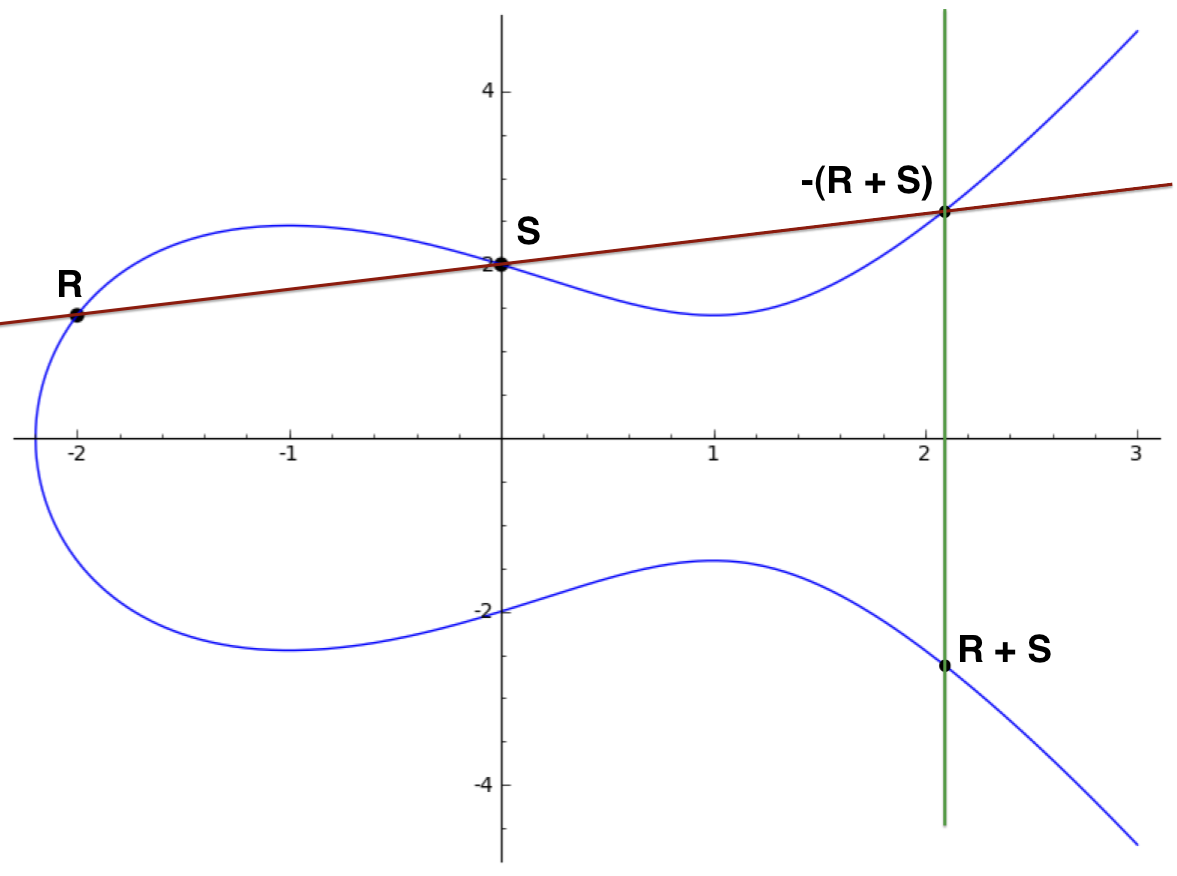
\includegraphics[scale=0.5]{figures/w_ells.png}
  \caption{$\ell_1$ and $\ell_2$ over a Weierstrass curve}
  \label{fig:w_ells}
\end{figure}

We can see the above claim that $g_{R, S} = \sfrac{\ell_1}{\ell_2}$ since
\[
div(\ell_1) = (R) + (S) + (-(R + S)) - 3(\mathcal{O})
\]
    because it has zeroes at $R$, $S$, and $-(R + S)$; since principal divisors
    have degree zero ($E$ is a smooth curve; see
    \cite{silverman2009arithmetic}, section II), we know that $\ell_1$ must
    have $\mathcal{O}$ as a pole of order three.
Similarly,
\[
div(\ell_2) = (-(R + S)) + (R + S) - 2(\mathcal{O})
\]
    since it intersects $E$ only at $R + S$, $-(R + S)$, and $\mathcal{O}$.
Finally,
\begin{align*}
div\left(\frac{\ell_1}{\ell_2}\right)
    &=  (R) + (S) + (-(R + S)) - 3(\mathcal{O}) -
            [(R + S) + (-(R + S)) - 2(\mathcal{O})]\\
    &=  (R) + (S) + (R + S) - (\mathcal{O})\\
    &=  div(g_{R, S})
\end{align*}
    as claimed.

This leads us to defining \textit{Miller functions} which arise in Miller's
    iterative algorithm for computing $\tau_n$.
We compute the needed $f$ with $div_P(f) = n(P) - n(\mathcal{O})$ with a take
    on the familiar ``double-and-and'' routine.
At each iteration we have some intermediate function $f_i$ with divisor $i(P) -
    (iP) - (i - 1)(\mathcal{O})$; after we complete our iterations, we have $f$
    since $nP = \mathcal{O}$.
This gives us Algorithm \ref{alg:miller}.

\begin{Algorithm}
\caption{Miller's Algorithm for computing $\tau_n$}
\label{alg:miller}
\begin{algorithmic}
    \Function{Miller}{$P, Q$}
        \State $f \gets 1$
        \State $R \gets P$
        \For{$i \gets k - 2 \texttt{ downto } 0$}
            \State $f \gets f^2 \cdot g_{R,R}(Q)$
            \State $R \gets 2R$ \Comment{Doubling Step}
            \If{$n_i = 1$}
                \State $f \gets f \cdot g_{R, P}(Q)$
                \State $R \gets R + P$ \Comment{Adding Step}
            \EndIf
        \EndFor
        \State $f \gets f^{\sfrac{(q^k - 1)}{n}}$
        \State \Return $f$
    \EndFunction
\end{algorithmic}
\end{Algorithm}

This algorithm is very efficient and the Weierstrass implementation has a nice
    geometric intuition behind it---the ``chord and tangent'' rule.
To compute pairings for a given normal form of an elliptic curve, it's enough
    to figure out what a Miller function looks like for that form, since this
    function ``forms the backbone for pairing computation.''
    \cite{das2008pairing}
Ergo in order to implement this for Edwards curves, we'll need a way to compute
    some Miller function $g_{R,S}$ with $div(g_{R,S}) = (R) + (S) - (R + S) -
    (\mathcal{O})$. 
So far pairing computations in the Edwards arena have been done for twisted
    Edwards curves, since they cover more cases of elliptic curves.
In trying to find Miller functions for binary Edwards curves, my research
    followed the same route that work has for twisted ones, beginning with the
    work of Das and Sarkar \cite{das2008pairing}.

\bodysection{Following Das \& Sarkar}

In \cite{das2008pairing}, the authors give a way of explicitly evaluating a
    pairing over twisted Edwards curves by using the birational map to and from
    a more familiar normal form.
We do the same here, but for binary Edwards curves.\footnote{In what follows,
    we shift our notation slightly to follow that of \cite{das2008pairing}
    instead of \cite{arene2011faster} since it makes our work slightly easier
    in the current setting.}

Let $\Phi$ be the birational map\footnote{It's really a group isomorphism when
    we extend it to the neutral elements, but nobody computes the pairing of a
    neutral element with another point in practice anyway.} from our binary
    Edwards curve $E$ to the corresponding Weierstrass curve
\[
W: v^2 + uv = u^3 + a_2u^2 + a_6
\]
Following the notation and work from \cite{moloneyefficient}, $\Phi$ is given
    by
\[
u = \sqrt{a_6}\left(\frac{(X + Y) Z}{d_1XY + d_1^2(X + Y)Z}\right)
\qquad
v = \sqrt{a_6}\left(\frac{(b + 1)XZ + bYZ}{d_1XY + d_1^2(X + Y)Z} + 1 +
    \frac{1}{d_1}\right)
\]
    where $b$ is chosen such that $b^2 + b = d_1^2 + d_2 + a_2$; i.e., $b$ is
    the half trace of $d_1^2 + d_2 + a_2$ (assuming that the degree $n$ of our
    binary field $\mathbb{F}_{2^n}$ is odd).
We also have $\Phi^{-1}: W \to E$ given by the projective coordinates
\begin{align*}
X   &=  d_1(bu + v + (d-1^2 + d_1)(d_1^2 + d_1 + d_2))\\
Y   &=  X + d_1u\\
z   &=  u^2 + d_1u + d_1^2(d_1^2 + d_1 + d_2)
\end{align*}

In order to calculate the pairing of $P_1$ and $P_2$ on $E$, we need to find a
    point $P_3$ and a rational function $h \in \mathbb{F}_{2^n}(E)$ such that
\[
\textrm{div}(h) = (P_1) + (P_2) - (P_3) - \mathcal{O}
\]
To do so, we'll map our points to $Q_1, Q_2, Q_3 \in W$ via $\Phi$, use the
    function
\[
g(u, v)
    =   \frac{\ell_1(u, v)}{\ell_2(u, v)}
    =   \frac{v + \lambda u + \theta}{u + u_3}
\]
    for lines $\ell_1$ through $Q_1$ and $Q_2$ and $\ell_2$ through $Q_3$ and
    $-Q_3$, then map back to $E$ via $\Phi^{-1}$.
The values $\lambda$ and $\theta$ are the slope and intercept of $\ell_1$,
    which is given via straight calculation.
Putting it all together, we have the following

\begin{thm}\label{thm:miller}
Let $E$ be a binary Edwards curve over $\mathbb{F}_{2^n}$ for $n$ odd, and $P_1
    = (X_1 : Y_1 : Z_1)$ and $P_2 = (X_2 : Y_2 : Z_2)$ be two points on $E$
    with sum $P_3 = (X_3 : Y_3 : Z_3)$.
Then the Miller function $h(x, y)$ such that
\[
\textrm{div}(h) = (P_1) + (P_2) - (P_3) - \mathcal{O}
\]
    is given by $\sfrac{N}{D}$, where
\[
D =
    (u1 + u2)
    (u_{3}  d_{1}  (d_{1} X Z + d_{1} Y Z + X Y) + \sqrt{a_6}  Z  (X + Y))
\]
    and the value of $N$ depends on whether $P_1$ and $P_2$ are equal:
\begin{enumerate}
\item   If $P_1 \ne P_2$, then 
\begin{align*}
N   &= Z  (X + Y)  d_{1}^{2}  (v_{1} u_{2} + u_{1} v_{2} + u_{1}
        \sqrt{a_6} + u_{2}\sqrt{a_6})\\
    &+ \sqrt{a_6}  (u_{1} + u_{2})  d_{1}  (X Y + X Z + Y Z)\\
    &+ Y  X  d_{1}  (v_{1} u_{2} + u_{1} v_{2})\\
    &+ \sqrt{a_6} (X Z u_{1} b + Y Z u_{1} b + X Z u_{2} b + Y Z u_{2} b\\
    &+ X Y u_{1} + X Z u_{1} + X Z v_{1} + Y Z v_{1} + X Y u_{2} + X Z u_{2} \\
    &+ X Z v_{2} + Y Z v_{2})\\
\end{align*}
\item If $P_1 = P_2$, then
\begin{align*}
N   &= u_{1}  Z  (X + Y)  d_{1}^{2}  (u_{1}^{2} + \sqrt{a_6})\\
    &+ u_{1}  d_{1}  (X Y u_{1}^{2} + X Y \sqrt{a_6} + X Z \sqrt{a_6} + Y Z
        \sqrt{a_6})\\
    &+  \sqrt{a_6}  (X Z u_{1}^{2} + Y Z u_{1}^{2} + X Z u_{1} b + Y Z u_{1} b
        + X Y u_{1} + X Z u_{1} + X Z v_{1} + Y Z v_{1})
\end{align*}
\end{enumerate}
\end{thm}

\begin{proof}
Given $\Phi(X, Y, Z) = (u, v)$ via the definition above, our function $h$ is
    $g\left(\Phi^{-1}(u, v)\right)$ per \cite{das2008pairing}.
That is, we have
\[
h
    =   g\left(
        \sqrt{a_6}\left(\frac{(X + Y) Z}{d_1XY + d_1^2(X + Y)Z}\right)
        ,
        \sqrt{a_6}\left(\frac{(b + 1)XZ + bYZ}{d_1XY + d_1^2(X + Y)Z} + 1 +
            \frac{1}{d_1}\right)
        \right)
\]
    which is equal to
\begin{equation}\label{eq:g_miller}
\frac{
    \sqrt{a_6}\left(
        \left[
            1 + \frac{1}{d_1} + \frac{(b + 1)XZ + bYZ}{d_1XY + d_1^2(X + Y)Z}
        \right]
        + \lambda\left[
            \frac{(X + Y)Z}{d_1XY + d_1^2(X + Y)Z}
        \right]
    \right) + \theta
}{
    \sqrt{a_6}\left[
        \frac{(X + Y)Z}{d_1XY + d_1^2(X + Y)Z} +
        \frac{(X_3 + Y_3)Z_3}{d_1X_3Y_3 + d_1^2(X_3 + Y_3)Z_3}
    \right]
}
\end{equation}
    where $\lambda$ and $\theta$ are determined by the line $\ell_1$.
Observe that if $P_1 \ne P_2$, then $\lambda$ is the slope of the line between
    them; if, on the other hand, $P_1 = P_2$, then it's the slope of the
    tangent line at $P_1$.
In either case, $\theta = v_1 + \lambda u_1$.

If $P_1 \ne P_2$, a straightforward calculation yields
\begin{equation}\label{eq:lam1}
\lambda = \frac{v_2 + v_1}{u_2 + u_1}
\end{equation}
    (since we're in characteristic two, addition and subtraction are the same).
If not, we use implicit differentiation on the equation for $W$ to find
    $\lambda = \frac{dv}{du}$:
\begin{align}\label{eq:lam2}
v^2 + uv = u^3 + a_6u^2 + a_2
    &\implies   2v\lambda + u\lambda + v = 3u^2 + 2a_6u\notag\\
    &\implies   \lambda\big\vert_{(u_1, v_1)} = \frac{u_1^2 + v_1}{u_1}
\end{align}
    remembering again that we're in characteristic two.

Replacing $\lambda$ with (\ref{eq:lam1}) and (\ref{eq:lam2}), in turn, and
    taking $\theta = v_1 + \lambda u_1$ yields the desired result after some
    tedious calculation.
Rather than show all the work, we include the following Sage script that
    will do the heavy lifting for us:
\lstinputlisting[caption={Calculations for binary Edwards Pairings},language=Python]{listings/calc.sage}
\end{proof}


\bodysection{Directions for Future Work}

Clearly the preceding theorem, though perfectly adequate, leaves something to
    be desired; a more elegant, cleaner solution for the Miller function would
    be nice.
The most clear way to such a solution, as evidenced by \cite{arene2011faster}
    and \cite{lipairing}, is to get a better understanding of the geometry of
    binary Edwards curves.
To that end, we show how to extend one of the theorems of
    \cite{arene2011faster} from twisted Edwards curves to binary Edwards
    curves.
We intend this theorem to be a stepping stone towards a full result similar to
    the main idea of \cite{arene2011faster}, wherein they give a new geometric
    formulation of the twisted Edwards curve group law (among many other
    interesting results).

In \cite{arene2011faster}, the authors give a new interpretation of the group
    law similar in its geometric flavor to the familiar ``chord-and-tangent''
    law of Weierstrass curves.
They show that the sum of two points on a twisted Edwards curve $E_{T, a, d}$
    can be given by a special conic: quoting their \textit{Remark 3}, ``we see
    that $P_1 + P_2$ is obtained as the mirror image with respect to the
    $y$-axis of the eighth intersection point of $E_{T, a,d}$ and the conic
    passing through $\Omega_1, \Omega_2, \mathcal{O}^\prime, P_1$, and $P_2$,''
    where $\Omega_1$ and $\Omega_2$ are the two points at infinity $(1 : 0 :
    0)$ and $(0 : 1 : 0)$, respectively, and $\mathcal{O}^\prime$ is the point
    $(0, -1)$ of order 2.
We offer an analogous result to their main theorem (1) that paves the way for
    their geometric interpretation in the hopes that it will inspire similar
    results for binary Edwards curves.

Let $\mathcal{O}^\prime = (1, 1) = (1 : 1 : 1)$; recall that this point has
    order 2.
Furthermore, let $\varphi(X, Y, Z) = c_{X^2}X^2 + c_{Y^2}Y^2 + c_{Z^2}Z^2 +
    c_{XY}XY + c_{XZ}XZ + c_{YZ}YZ \in K[X, Y, Z]$ be a homogeneous polynomial
    of degree 2 and $C: \varphi(X, Y, Z) = 0$ be the associated plane (possibly
    degenerate) conic.
Like in \cite{arene2011faster}, since the points $\Omega_1, \Omega_2,$ and
    $\mathcal{O}^\prime$ do not lie on a line, a conic $C$ passing through
    these points cannot be a double line and $\varphi$ represents $C$ uniquely
    up to multiplication by a scalar.
By evaluating $\varphi$ at $\Omega_1, \Omega_2,$ and $\mathcal{O}^\prime$, we
    get the following:
\begin{align*}
\Omega_1:\qquad &\varphi(1 : 0 : 0) = c_{X^2}\\
\Omega_2:\qquad &\varphi(0 : 1 : 0) = c_{Y^2}\\
\mathcal{O}^\prime:\qquad&\varphi(1, 0, 0) = c_{X^2} + c_{Y^2} + c_{Z^2} +
                                             c_{XY} + c_{XZ} + c_{YZ}
\end{align*}
Hence $c_{X^2} = c_{Y^2} = 0$ and $c_{Z^2} = c_{XY} + c_{XZ} + c_{YZ}$.
Therefore $C$ must have the form:
\begin{equation}\label{eq_C}
c_{XY}(XY + Z^2) + c_{XZ}(XZ + Z^2) + c_{YZ}(YZ + Z^2)
\end{equation}
Next we have the following analogous result to Theorem 1 of
    \cite{arene2011faster}:

\begin{thm}\label{thm:arene}
Let $E_{B, d_1, d_2}$ be a binary Edwards curve over $K$ and let $P_1 = (X_1 :
    Y_1 : Z_1)$ and $P_2 = (X_2 : Y_2 : Z_2)$ be two affine, not necessarily
    distinct, points on $E_{B, d_1, d_2}(K)$.
Let $C$ be the conic passing through $\Omega_1, \Omega_2, \mathcal{O}^\prime,
    P_1,$ and $P_2$ which must have the form (\ref{eq_C}).
If some of the above points are equal, we consider $C$ and $E_{B, d_1, d_2}$
    to intersect with at least that multiplicity at the corresponding point.
Then the coefficients in (\ref{eq_C}) of the equation $\varphi$ of the conic
    $C$ are uniquely determined (up to scalars) as follows:
\begin{enumerate}
\item
If $P_1 \ne P_2, P_1 \ne \mathcal{O}^\prime,$ and $P_2 \ne \mathcal{O}^\prime$,
    then
\begin{align*}
c_{XY}  &=Z_1Z_2\left[X_1(Y_2 + Z_2) + Y_1(X_2 +Z_2) + Z_1(X_2 + Y_2)\right]\\
c_{XZ}  &=Y_1Z_2(X_1Y_2 + X_1Z_2 + Z_1Z_2) + Y_2Z_1(Y_1X_1 + Z_1X_1 + Z_1Z_2)\\
c_{YZ}  &=X_1Z_2(Y_1X_2 + Y_1Z_2 + Z_1Z_1) + X_2Z_1(X_1Y_2 + Z_1Y_2 + Z_1Z_2)
\end{align*}
\item
If $P_1 \ne P_2 = \mathcal{O}^\prime$, then $c_{XY} = Z_1, c_{XZ} = Z_1,$ and
    $c_{YZ} = X_1 $
\item
If $P_1 = P_2$, then
\begin{align*}
c_{XY}  &=  X_1^2Y_1 + X_1Y_1^2 + d_1X_1Z_1^2 + X_1^2Z_1 + d_1Y_1Z_1^2 +
            Y_1^2Z_1 + X_1Z_1^2 + Y_1Z_1^2\\
c_{XZ}  &=  X_1^2Y_1 + d_1Y_1^2Z_1 + X_1Y_1^2 + d_1X_1Z_1^2 + X_1^2Z_1\\
        &+ d_1Y_1Z_1^2 + X_1Y_1Z_1 + d_1Z_1^3 + Y_1Z_1^2\\
c_{YZ}  &=  d_1X_1^2Z_1 +d_2X_1^2Z_1 + d_2Y_1^2Z_1 + X_1^2Z_1 + d_1Z_1^3 +
            X_1Z_1^2
\end{align*}
\end{enumerate}
\end{thm}

\begin{proof}
We tackle each case separately.
\begin{enumerate}
\item
If the points $P_1$ and $P_2$ are distinct, evaluating equation \ref{eq_C} at
    the two points yields two linear equations in the coefficients:
\begin{align*}
c_{XY}(X_1Y_1 + Z_1^2) + c_{XZ}(X_1Z_1 + Z_1^2) + c_{YZ}(Y_1Z_1 + Z_1^2) &= 0\\
c_{XY}(X_2Y_2 + Z_2^2) + c_{XZ}(X_2Z_2 + Z_2^2) + c_{YZ}(Y_2Z_2 + Z_2^2) &= 0
\end{align*}
Since we're working in projective coordinates, two equations is enough to
    uniquely determine the three unknowns, and we get the following solutions:
\begin{align*}
c_{XY}
    &=  \begin{vmatrix}
        X_1Z_1 + Z_1^2  &   Y_1Z_1 + Z_1^2\\
        X_2Z_2 + Z_2^2  &   Y_2Z_2 + Z_2^2
        \end{vmatrix}\\
    &=  (X_1Z_1 + Z_1^2)(Y_2Z_2 + Z_2^2) + (X_2Z_2 + Z_2^2)(Y_1Z_1 + Z_1^2)\\
    &=  Z_1Z_2\left[X_1(Y_2 + Z_2) + Y_1(X_2 +Z_2) + Z_1(X_2 + Y_2)\right]\\
c_{XZ}
    &=  \begin{vmatrix}
        X_1Y_1 + Z_1^2  &   Y_1Z_1 + Z_1^2\\
        X_2Y_2 + Z_2^2  &   Y_2Z_2 + Z_2^2
        \end{vmatrix}\\
    &=  (X_1Y_1 + Z_1^2)(Y_2Z_2 + Z_2^2) + (X_2Y_2 + Z_2^2)(Y_1Z_1 + Z_1^2)\\
    &=  X_1^2Y_1 + d_1Y_1^2Z_1 + X_1Y_1^2 + d_1X_1Z_1^2 + X_1^2Z_1\\
    &+ d_1Y_1Z_1^2 + X_1Y_1Z_1 + d_1Z_1^3 + Y_1Z_1^2\\
c_{YZ}
    &=  \begin{vmatrix}
        X_1Y_1 + Z_1^2  &    X_1Z_1 + Z_1^2\\
        X_2Y_2 + Z_2^2  &    X_2Z_2 + Z_2^2
        \end{vmatrix}\\
    &=  (X_1Y_1 + Z_1^2)(X_2Z_2 + Z_2^2) + (X_2Y_2 + Z_2^2)(X_1Z_1 + Z_1^2)\\
    &=  d_1X_1^2Z_1 +d_2X_1^2Z_1 + d_2Y_1^2Z_1 + X_1^2Z_1 + d_1Z_1^3 + X_1Z_1^2
\end{align*}
    as claimed.

\item
Note that $C$ is tangent to the curve $E_{B, d_1, d_2}$ at the point
    $\mathcal{O}^\prime$ if and only if $0 = \left(\sfrac{\partial\varphi}
    {\partial x}\right)(1 : 1 : 1) = c_{XY} + c_{XZ}$, i.e. iff $c_{XY} =
    c_{XZ}$.
Then
\[
\varphi
    =   c_{XY}(XY + Z^2 + XZ + Z^2) + c_{YZ}(YZ + Z^2)
    =   (Y + Z)(c_{XY}X + c_{YZ}Z)
\]
Since $P_1 \ne \mathcal{O}^\prime$, it doesn't lie on the line $Y + Z = 0$, so
    $c_{XY}X_1 + c_{YZ}Z_1 = 0$.
Then together $c_{XY} = c_{XZ}$ and $c_{XY}X_1 = c_{YZ}Z_1$ imply the result.

\item
In the final case, let $Z = Z_1 = 1$ in our equations.
The tangent vectors at $P_1 = (X_1 : Y_1 : 1) = (X_1, Y_1)$ of
    $E_{B, d_1, d_2}$ and $C$ are
\[
\begin{pmatrix}
    \sfrac{\partial E}{\partial Y} \\ \sfrac{\partial E}{\partial X}
\end{pmatrix}
=   
\begin{pmatrix}
d_1 + X_1 + X_1^2 \\ d_1 + Y_1 + Y_1^2
\end{pmatrix}
\qquad
\begin{pmatrix}
    \sfrac{\partial C}{\partial Y} \\ \sfrac{\partial C}{\partial X}
\end{pmatrix}
\begin{pmatrix}
c_{XY}X_1 + c_{YZ} \\ c_{XY}Y_1 + c_{XZ}
\end{pmatrix}
\]
    (note that we can drop the usual negative signs because $\textrm{char}(K) =
    2$).
These vectors are collinear if and only if
\begin{align*}
0
    &=  \begin{vmatrix}
        d_1 + X_1 + X_1^2   &   c_{XY}X + c_{YZ}\\
        d_1 + Y_1 + Y_1^2   &   c_{XY}Y + c_{XZ}
        \end{vmatrix}\\
    &=  c_{XY}(d_1Y_1 + X_1Y_1 + X_1^2Y_1 + d1X_1 + X_1Y_1 + X_1Y_1^2)\\
    &+c_{XZ}(d_1 + X_1 + X_1^2) + c_{YZ}(d_1 + Y_1 + Y_1^2)\\
    &=  c_{XY}(d_2(X_1^2 + Y_1^2) + X_1^2Y_1^2) +
        c_{XZ}(d_1 + X_1 + X_1^2) +
        c_{YZ}(d_1 + Y_1 + Y_1^2)
\end{align*}
    using the curve equation to simplify.
We also know that
\[
0   =   \varphi(X_1, Y_1, 1)
    =   c_{XY}(X_1Y_1 + 1) + c_{XZ}(X_1 + 1) + c_{YZ}(Y_1 + 1)
\]
These two equations can be solved in the same manner as our work in the first
    case, yielding
\begin{align*}
c_{XY}
    &=  \begin{vmatrix}
        d_1 + X_1 + X_1^2   &   d_1 + Y_1 + Y_1^2\\
        X_1 + 1   &   Y_1 + 1
        \end{vmatrix}\\
    &=  d_1(X_1 + Y_1) + X_1 + Y_1 + X_1^2 + Y_1^2 + X_1^2Y_1 + X_1Y_1^2\\
    &=  (X_1 + Y_1)(X_1Y_1 + X_1 + Y_1 + d_1 + 1)
\end{align*}
    for the first coefficient,
\begin{align*}
c_{XZ}
    &=  \begin{vmatrix}
        d_2(X_1^2 + Y_1^2) + X_1^2Y_1^2 &   d_1 + Y_1 + Y_1^2\\
        X_1Y_1 + 1  &   Y_1 + 1
        \end{vmatrix}\\
    &=  d_1(X_1Y_1 + 1) + d_2(X_1^2Y_1 + Y_1^3 + X_1^2 + Y_1^2) + X_1^2\\
    &+ Y_1^2 + X_1Y_1^2 + X_1Y_1^3 + Y_1 + Y_1^2 + X_1^2Y_1^3\\
    &=  X_1^2Y_1 + d_1Y_1^2 + X_1Y_1^2 + d_1X_1 + X_1^2 + d_1Y_1 + X_1Y_1 + d_1
        + Y
\end{align*}
    for the second, and
\begin{align*}
c_{YZ}
    &=  \begin{vmatrix}
        d_2(X_1^2 + Y_1^2) + X_1^2Y_1^2 &   d_1 + X_1 + X_1^2\\
        X_1Y_1 + 1  &   X_1 + 1
        \end{vmatrix}\\
    &=  d_1(X_1Y_1 + 1) + d_2(X_1^3 + X_1^2 + X_1Y_1^2 + Y_1^2) + X_1^34Y_1^2\\
    &+ X_1^2Y_1^2 + X_1^2Y_1 + X_1^3Y_1 + X_1 + X_1^2\\
    &=  d_1X_1^2 + d_2X_1^2 + d_2Y_1^2 + X_1^2 + X_1 + d_1
\end{align*}
    for the third, using the curve equation to simplify.
Homogenizing yields the stated result.
Note that the same formulas work if $P_1 = \mathcal{O}^\prime$, since then we
    still have $\varphi = 0$.\qedhere
\end{enumerate}
\end{proof}

Unfortunately, it's not entirely clear where to go from here; the geometry of
    twisted Edwards curves is different from the geometry of binary Edwards
    curves.
Moreover, though working in characteristic two has some benefits to arithmetic,
    more often than not it seems to complicate calculations.
Therefore, theorem \ref{thm:arene} is offered as a possible starting point for
    future research instead of an end in and of itself.
If we were to continue to mirror the progression of results for pairings on
    twisted Edwards curves, the next step would be to expand on a result
    similar to \cite{arene2011faster}'s to get one similar to
    \cite{lipairing}'s.
Again, because the geometry of binary Edwards curves differs so much from that
    of twisted means the results of this paper don't directly apply, but they
    do offer an intriguing possibility for another direction.
Such a result would involve not only reinterpreting the geometry of binary
    Edwards curves, but would also involve working in extended coordinates
    (four instead of the usual three for projective space).

\bodychapter{Applications}
\label{chp:app}

In this chapter we discuss two applications of elliptic curve cryptography,
    both of which benefit from the added security granted by the binary Edwards
    group law.
Moreover, they may be more attractive to implementors because they use binary
    Edwards curves rather than some other type; computers do work in binary,
    after all, so binary Edwards curves can lend themselves to efficient
    implementation in software or even hardware (e.g.
    \cite{chatterjee2011fpga}, \cite{kocabas2009hardware},
    \cite{kocabas2010implementation}).

\bodysection{Password Based Key Derivation}

\bodysubsection{Background}
Our first application is a password based key derivation function, or PBKDF.
Password safety is paramount in today's interconnected world; users log in to
    multiple workstations, websites, and services for communication, work,
    banking---the list goes on.
Despite its importance, password safety still a tricky technical subject, one
    that even experts get wrong sometimes; for example, according to
    \cite{arstechnica}, the IEEE exposed plaintext passwords in a public FTP
    directory ``for over a month.''
One way to securely store passwords is, somewhat paradoxically, to not store
    them at all.
Instead, a system can use a PBKDF to store different information derived from a
user's login credentials to authenticate them.

To quote \cite{percival2009stronger},
\begin{quote}
Password-based key derivation functions are used for two primary purposes:
    First, to hash passwords so that an attacker who gains access to a password
    file does not immediately possess the passwords contained therein; and
    second, to generate cryptographic keys to be used for encrypting and/or
    authenticating data.
\ldots Since all modern key derivation functions are constructed from hashes
    against which no non-trivial pre-image attacks are known, attacking the key
    derivation function directly is infeasible; consequently, the best attack
    in either case is to iterate through likely passwords and apply the key
    derivation function to each in turn.
Unfortunately, this form of ``brute force'' attack is quite liable to succeed.
Users often select passwords which have far less entropy than is typically
    required of cryptographic keys; a recent study found that even for web
    sites such as \texttt{paypal.com}, where---since accounts are often linked
    to credit cards and bank accounts---one would expect users to make an
    effort to use strong passwords, the average password has an estimated
    entropy of 42.02 bits, while only a very small fraction had more than 64
    bits of entropy.\footnote{The cited study is \cite{florencio2007large}.}
This is where a properly designed PBKDF comes in.
\end{quote}

As \cite{turan2010recommendation} says, ``the main idea of a PBKDF is to slow
    dictionary or brute force attacks on the passwords by increasing the time
    needed to test each password.''
Ideally, it should behave like a random mapping from passwords to possible
    data, which we'll called \textit{password hashes}, though this term is
    somewhat problematic.\footnote{Using ``hashes'' may lead one to think that
    using a general-purpose hash function like SHA-256 as a PBKDF is a good
    idea; as we'll see, this is not the case.}
To slightly borrow some of \cite{menezes1996handbook}'s exposition, ``a
    password, associated with each user (entity), is typically a string of 6 to
    10 or more characters the user is capable of committing to memory.''
In order to authenticate herself to the system in question, ``the user enters a
    (userid, password) pair'' to the system, which then uses this information
    in some way to compute the hash.
Once this computation is complete, the system checks the hash against the
    credentials it has stored for the supplied userid; if the hash matches the
    one on file, the user is granted access to the system.

Clearly a string of 6 to 10 memorable characters may not have enough entropy to
    qualify as cryptographically secure; therefore, a PBKDF should be designed
    to make the hash output look as random as possible.
Randomness alone isn't enough, however; as \cite{percival2009stronger} mentions
    above, cryptographic security can be compromised if the PBKDF is too
    computationally simple to perform; consider the following example.
\begin{ex}
Suppose an eavesdropper Eve manages to get her hands on the table of
\[
[\mathrm{userid}, \mathrm{hash}(\mathrm{password})]
\]
    pairs for Alice's system.
If Eve's desire to break into Alice's system isn't particularly time sensitive,
    she can simply grab a large file of likely passwords and hash them all
    until she finds a match in the second column of the table.
If Alice chose to use a general purpose message hashing algorithm for her
    PBKDF like SHA-3 (\cite{baum2012nist}), Eve may have the computational
    power to break into Alice's system soon enough to cause severe damage.
\end{ex}

One way to combat this ``dictionary attack'' is to widen the search space by
    \textit{salting} the hashes; for each userid, a system may instead store
    $\mathrm{hash}(\mathrm{password} \ast \mathrm{salt})$ for some operation
    $\ast$, typically string concatenation or bit exclusive-or, where the salt
    is a secret value known only to the system.
In this setup, a potential attacker would have to brute-force over all possible
    salts as well as all possible passwords, greatly increasing the work
    involved.
Even with salting, however, the speed of hash can still be an issue given
    today's technology.
There are a number of recent publications regarding cracking password hashes by
    brute force, many of which use the advanced parallel computing power
    granted by today's GPUs---see \cite{alnoonexecuting,
    gomez2010cryptanalysis, lim2004parallelization}, and
    \cite{zonenberg2009distributed}.

To make matters worse, the inevitable increase in computing power we experience
    as technology changes means that attackers will be able to attack any fixed
    PBKDF more and more easily as time goes by.
This means that a successful PBKDF should be tunable to meet this rising power
    available to would-be password crackers; as \cite{provos1999future} puts
    it, we are looking for a future-adaptable password scheme to ``keep up with
    hardware speeds.''
A secure PBKDF's computational cost ``must increase as hardware improves.''

One other successful PBKDF is \cite{provos1999future}'s \texttt{bcrypt}.
However, it isn't the final answer to the PBKDF problem; \texttt{bcrypt} is
    already under some scrutiny, and some alternatives have been proposed, the
    most notable of which is probably \cite{percival2009stronger}'s
    \texttt{scrypt}.
Like \texttt{scrypt}, our proposed PBKDF will incorporate a pseudorandom
    number generator.
It will also make use of binary Edwards curves; although they can be
    implemented rather efficiently, the inherent complexity of binary Edwards
    curves compared to the computer primitives of which typical hash functions
    are built adds to the security of our PBKDF.

\bodysubsection{Proposed PBKDF}
To further research into and development of secure PBKDFs, I propose we take a
    cue from NIST: look at a candidate scheme that is very different
    from what currently exists, so they won't (necessarily) be vulnerable to
    the same attacks, like NIST did with the recent SHA-3 competition.
Explaining some of the reasons for declaring \texttt{Keccak} the winner, they
    wrote
    \begin{quote}
    ``Keccak has the added advantage of not being vulnerable in the same ways
    SHA-2 might be,''says NIST computer security expert Tim Polk. ``An attack
    that could work on SHA-2 most likely would not work on Keccak because the
    two algorithms are designed so differently.'' \cite{baum2012nist}
    \end{quote}
In fact, we'll take even more from NIST's recent competition and present a
    variation on the Elliptic Curve Only Hash (ECOH, \cite{brown2008ecoh})
    which was submitted to the SHA-3 competition in 2008.
This variation makes some changes to the original algorithm to combat the
    main weakness that lost it the competition, viz. the second pre-image
    attack found in \cite{halcrow2009second, cryptoeprint:2009:168}.
At the same time, these changes ensure that while several different instances
    of our PBKDF can be parallelized, the algorithm itself is inherently serial
    and thus resists any further attempts at parallelization.

Specifically, the points $P_i$ and the values $X_1$ and $X_2$ presented in this
    section rely on the state of the algorithm at every step.
That is, each $P_i$ for $i > 0$ relies upon the previous $P_{i-1}$, and both
    $X_1$ and $X_2$ rely on the all of the $P_i$.
We also incorporate a pseudorandom number generator, not unlike other PBKDFs
    like \texttt{scrypt} \cite{percival2009stronger}.
As mentioned, these changes effectively ameliorate the second pre-image attack
    from \cite{cryptoeprint:2009:168}; they also have force the different
    stages of the hash to be computed serially, removing any chance of
    parallelization.
This makes our PBKDF more resilient in the face of processors that are no
    longer scaling up to greater speeds but out to more and more cores; for an
    offline attack, only multiple instances of our PBKDF can be run on a
    parallel machine or GPU.
The PBKDF itself can't be sped up.

Finally, we make some changes to the parameters involved.
Rather than sticking to an Elliptic curve in Weierstrass form, we make use of
    a binary Edwards curve; this makes the PBKDF more resistant to side-channel
    analysis.
We also remove the nondeterministic part of the \textit{Search} step of ECOH,
    instead using the ideas from \cite{icart2009hash} to deterministically map
    a field element to a point on our curve.
In doing so, we incorporate the birational map from \cite{moloneyefficient}.

Our PBKDF, called \texttt{ECOH's Echo}, takes in a salt $s$ and password $p$
    and makes use of the following parameters:
\begin{itemize}
\item   a pseudorandom number generator PRNG that can be seeded (primed with an
initial state)
\item   a block size $blen$, number of blocks/rounds $numblocks$, length $ilen$
    for integer bit representations, and an output length
\item   a finite field $\mathbb{F}_{2^n}$, an algebraic extension of
    $\mathbb{F}_2$ of degree $n$
\item   $a_2$ and $a_6$, two elements of $\mathbb{F}_{2^n}$ determining an
    elliptic curve in Weierstrass form
\item   $E$, the birationally equivalent binary Edwards curve
\item   $G$, a base point on $E$
\end{itemize}
Note that our parameters are not set in stone, but rather can be scaled up to
    larger sizes as potential attacking computing power increases.
We can increase our degree $n$ as well as the other parameters as the need
    arises.

We also make use of a number of maps:
\begin{itemize}
\item   $\pi$, a deterministic map from $K$ to $E$ (see \cite{icart2009hash}
    and \cite{moloneyefficient}) that takes a fixed number of steps
\item   A mapping $\omega: E \times \{X, Y\} \to K$, given by
\[
(Q, Z) \mapsto \frac{\left\lfloor Q + \left\lfloor \frac{Q.z}{2} \right\rfloor
    G \right\rfloor.z}{2} \bmod 2^{blen}
\]
    where $z = x$ if $Z = X$ and $y$ if $Z = Y$ (i.e., $Z$ picks out the
    coordinate).
This is an extension of the output mapping from the original ECOH submission
    (\cite{brown2008ecoh}) to work with either of a point's coordinates.
\item   A mapping $\varphi: E \to K$ given by $\varphi(Q) = \omega(Q, X)$ (not
    strictly needed, of course, this is just a specialization of $\omega$)
\item   A mapping $\psi: E \to \mathbb{F}_2$ given by $\psi(Q) = \omega(Q, Y)
    \& 1$, the least significant bit of $\omega(Q, Y)$
\end{itemize}
Before we move on, let's flesh out the details of the map $\pi$.
Take \cite{icart2009hash}'s $f_{a_2, a_6}:\mathbb{F}_{2^n} \to
    W(\mathbb{F}_{2^n})$ where $W$ is an elliptic curve in the Weierstrass form
\[
v^2 + uv = u^3 + a_2u^2 + a_6
\]
    defined by $z \mapsto (u, v)$ such that
\begin{align*}
\alpha  &=  a_2 + z + z^2\\
u       &=  (\alpha^4 + \alpha^3 + a_6)^{\sfrac{1}{3}} + \alpha\\
v       &=  zu + \alpha^2
\end{align*}
    and combine it with \cite{moloneyefficient}'s birational equivalence to
    create $\pi$ via $z \mapsto (u, v) \mapsto (x, y)$.\footnote{We use this
    one instead of the original given in \cite{bernstein2008binary} due to its
    having only one exceptional point ($\infty$ which won't show up here) and
    being more efficient in implementation.} 
This gives us a direct mapping $\pi: \mathbb{F}_{2^n} \to E(\mathbb{F}_{2^n})$
    that inherits all of the cryptographically desirable properties of
    $f_{a_2, a_6}$ since the birational equivalence has no exceptional points
    save $\infty$.
Moreover, it's more secure than the \textit{Search} step of ECOH, since this
    was a nondeterministic map that would take an indeterminate amount of
    steps.
As always, we strive to minimize the leakage of extra information through
    side-channels.

We'll first give a more na\"ive version of \texttt{ECOH's Echo}.

\bodysubsubsection{Na\"ive Version}
Execution proceeds as follows: first, our PRNG is seeded with the exclusive-or
    (XOR) of the password and salt.\footnote{Strictly speaking, there is an
    encoding involved in making an integer value out of the password. In our
    reference implementation below, we make the usual choice of treating the
    password as a string of ASCII-encoded bytes and build an integer out of
    that.}
Each block $O_i$ is generated in the following way: given an integer $i$,
    append the $ilen$-bit representation of $i$ to a $blen - ilen$ long stream
    of pseudorandom bits from PRNG.
Second, we initialize a point $P_0$ from the initial block $O_0$ by setting it
    to be $\pi(O_0)$.
We then iterate for $numblocks - 1$ rounds, setting $P_i$ to be $\pi(O_i \oplus
    i \oplus \varphi(P_{i-1}))$.
Next we update $numblocks$, saving
\[
numblocks \oplus \left(\sum\nolimits_0^{numblocks - 1}2^i\psi(P_i)\right)
\]
    in its place.
After that, $X_1$ and $X_2$ are defined to be $\pi(numblocks)$ and
\[
\pi\left(numblocks \oplus
    \left[\bigoplus\nolimits_0^{numblocks-1} O_i\right]
\right)
\]
    respectively.
Finally, we define $Q$ to be the sum
\[
X_1 + X_2 + \sum\nolimits_0^{numblocks-1}P_i
\]
    and output $\varphi(Q)$.

\bodysubsubsection{Memory Efficient Version}
Though it's simpler to follow, the above version of our PBKDF is not as
    efficient with regards to memory as it could be.
We needn't store all the intermediate points $P_i$, for instance, if we instead
    introduce two temporary variables $Y_1$ and $Y_2$ that will be used to
    build $X_1$ and $X_2$ later.
After seeding PRNG as before, let $(O, Y_1, Y_2) = (O_0, numblocks, numblocks)$
    and set $Q = P = \pi(O)$.
Then we iterate for $i \in \{1, \ldots, numblocks - 1\}$, setting
\begin{align*}
O   &=  O_i\\
P   &=  \pi(O \oplus i \oplus \varphi(P))\\
Y_1 &=  Y_1 + 2^i\psi(P)\\
Y_2 &=  Y_2 \oplus O\\
Q   &=  Q + P
\end{align*}
    at each step of the loop.
Finally, let $X_1 = \pi(Y_1)$, $X_2 = \pi(Y_1 \oplus Y_2)$, and $Q = Q + X_1 +
    X_2$.
As before, we output $\varphi(Q)$.

\bodysubsection{Algorithm Pseudocode and Diagrams}
We give a description of \texttt{ECOH's Echo} in algorithms (\ref{alg:naive})
    and (\ref{alg:good}).
Diagrams of the flow of the rounds in the more efficient description are given
    in Figures (\ref{fig:first_round}) and (\ref{fig:other_rounds}).

\begin{Algorithm}
\caption{ECOH's Echo, Na\"ive version}
\label{alg:naive}
\begin{algorithmic}
    \Function{ECOH's Echo}{$p, s$}
        \State PRNG.salt$(s \oplus p)$
        \State $P_0 \gets \pi(O_0)$
        \For{$i \gets 1 \texttt{ to } numblocks - 1$}
            \State $P_i \gets \pi\left(O_i \oplus i \oplus
                \varphi(P_{i-1})\right)$
        \EndFor
        \State $numblocks \gets numblocks \oplus \left(\sum_0^{numblocks - 1}
            2^i\psi(P_i)\right)$
        \State $X_1 \gets \pi(numblocks)$
        \State $X_2 \gets \pi\left(numblocks \oplus
            \left[\bigoplus_0^{numblocks-1} O_i\right]\right)$
        \State $Q \gets X_1 + X_2 + \sum_0^{numblocks-1}P_i$
        \State \Return $\varphi(Q)$
    \EndFunction
\end{algorithmic}
\end{Algorithm}

\begin{Algorithm}
\caption{ECOH's Echo, Memory-Efficient Version}
\label{alg:good}
\begin{algorithmic}
    \Function{ECOH's Echo}{$p, s$}
        \State PRNG.salt$(s \oplus p)$
        \State $O \gets O_0$
        \State $Y_1 \gets numblocks$
        \State $Y_2 \gets numblocks$
        \State $P \gets \pi(O)$
        \State $Q \gets P$
        \For{$i \gets 1 \texttt{ to } numblocks - 1$}
            \State $O \gets O_i$
            \State $P \gets \pi\left(O \oplus i \oplus \varphi(P)\right)$
            \State $Y_1 \gets Y_1 \oplus 2^i\psi(P)$
            \State $Y_2 \gets Y_2 \oplus O$
            \State $Q \gets Q + P$
        \EndFor
        \State $X_1 \gets \pi(Y_1)$
        \State $X_2 \gets \pi\left(Y_1 \oplus Y_2\right)$
        \State $Q \gets Q + X_1 + X_2$
        \State \Return $\varphi(Q)$
    \EndFunction
\end{algorithmic}
\end{Algorithm}

\begin{figure}[htbp]
    \centering
    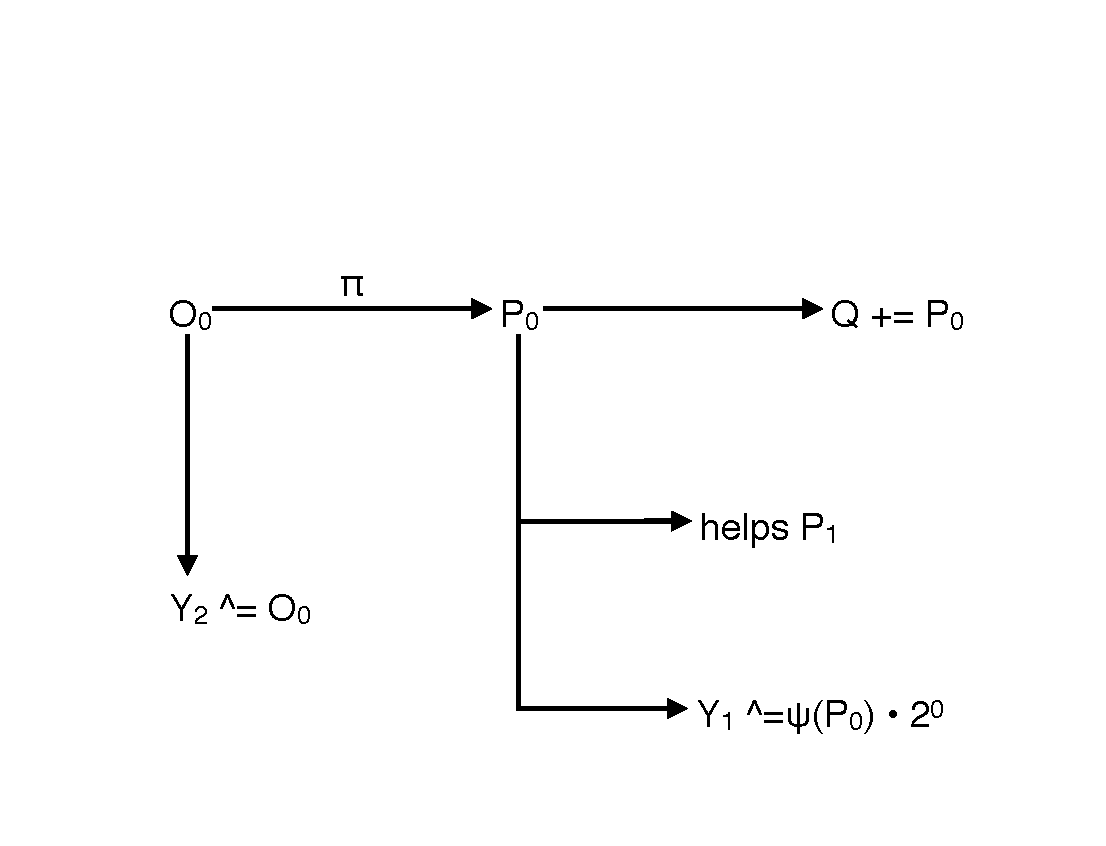
\includegraphics[scale=0.5]{figures/ecoh_echo.pdf}
    \caption{First round of \texttt{ECOH's Echo}}
    \label{fig:first_round}
\end{figure}

\begin{figure}[htbp]
    \centering
    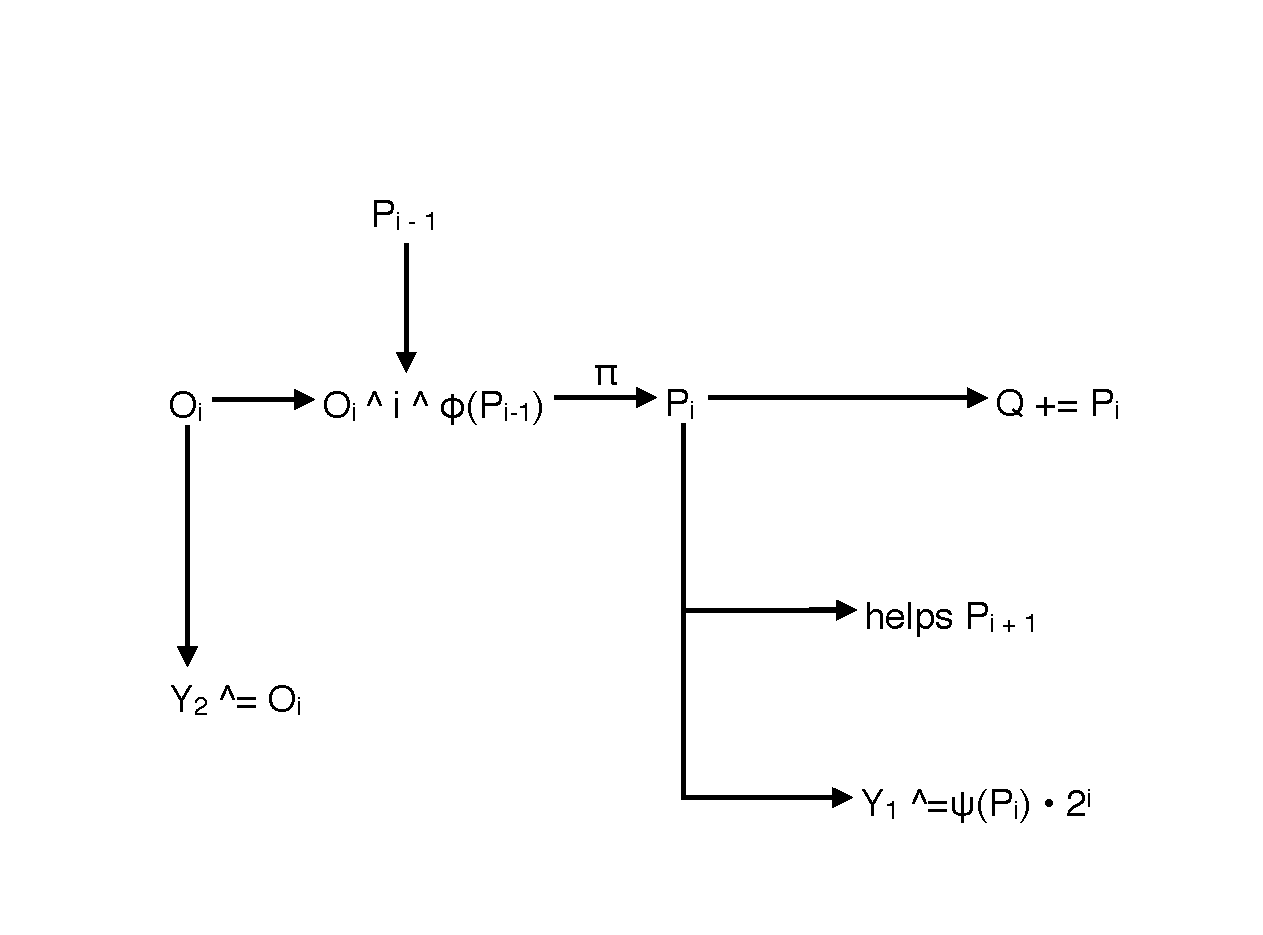
\includegraphics[scale=0.5]{figures/ecoh_echo2.pdf}
    \caption{Subsequent rounds of \texttt{ECOH's Echo}}
    \label{fig:other_rounds}
\end{figure}

\newpage
\bodysubsection{\texttt{ECOH's Echo} Reference Implementation}
Finally, we provide a reference implementation of \texttt{ECOH's Echo} using
    our software library \texttt{e2c2}.
For more on \texttt{e2c2}, see Appendix \ref{chp:src}.
\lstinputlisting[caption={ECOH's Echo}]{backmatter/src/ecoh_echo.cc}

\bodysection{Compartmented ID-Based Secret Sharing and Signcryption}

Another application of elliptic curves and elliptic curve cryptography is using
    pairings for identity-based schemes, like those first suggested in
    \cite{boneh2001identity}.\footnote{A previous of this section has been
    posted to the International Association for Cryptologic Research's
    cryptology eprint archive (\texttt{http://eprint.iacr.org/2012/528}) and
    has been submitted for consideration to the Information Processing Letters
    Journal for consideration for publication.}
In \cite{li2006id}, Li, Xin, and Hu describe an ID-based signcryption scheme
    that uses a bilinear map to accomplish $(t, n)$ shared unsigncryption with
    the help of Shamir's secret sharing scheme.
Here we describe a way to extend Li et. al.'s construction into a
    \textit{compartmented scheme}.
For our compartmented scheme, suppose the organization $\mathcal{O}$ is split
    into several compartments $\mathcal{C}_i$, $i \in \{1, \ldots, t\}$.
In order to unsigncrypt a message sent to $\mathcal{O}$, at least one member of
    each of the $t$ compartments must participate; without the cooperation of
    at least one member from each compartment, the message cannot be
    unsigncrypted.
What's more, each member $\mathcal{M}_{ij} \in \mathcal{C}_i$ gets
    different information; therefore, although any $\mathcal{M}_{ij}$ can
    participate equally, the compartment $\mathcal{C}_i$ is in fact split up
    so that all of its potential participants have something unique to
    contribute.

In what follows, we will make the following changes to the terminology and
    notation of \cite{li2006id}: uppercase letters will denote points on an
    elliptic curve $E$ over a predetermined finite field $K$, lowercase letters
    will denote elements in the multiplicative group $\mu_n$ of $n$th roots of
    unity, Greek letters are used for elements of $\mathbb{F}_q$, and script
    letters generally denote compartments or members thereof.
Moreover, $\widehat{e}$ is a pairing function from $E \times E \to \mu_n =
    \mathbb{F}_{q^k}^\ast/\mathbb{F}_{q^k}^{\ast n}$.

\bodysubsection{Preliminaries}
Here we briefly discuss the basic tools needed for our scheme, namely
\begin{enumerate}
\item Bilinear Diffie-Hellman Problems
\item Identity-based encryption
\item Shamir's threshold scheme
\item Signcryption
\item Baek \& Zheng's zero knowledge proof for the equality of two discrete
    logarithms based on a bilinear map
\end{enumerate}
We also cite relevant references for readers who would like more in-depth
    coverage of these interesting topics.

\bodysubsubsection{Bilinear Diffie-Hellman Problems}
As \cite{menezes1996handbook} writes, bilinear maps were first used in
    cryptography to weaken systems rather than create them.
In \cite{menezes1993reducing}, the authors showed that ``the discrete logarithm
    problem for an elliptic curve over a finite field $\mathbb{F}_q$ can be
    reduced to the discrete logarithm problem in some extension field
    $\mathbb{F}_q^k$.''
For a particular class of curves called \textit{supersingular} curves, this was
    a particularly devastating attack.
Fortunately for elliptic curve cryptography, not all curves are supersingular.

The basic idea behind this attack was that if $Q = \ell P$, then
\[
\widehat{e}(P, Q)
    = \widehat{e}(P, P)^\ell 
\]
    so we can solve the resulting discrete logarithm problem (or Diffie-Hellman
    problem) in a different group instead, one where logarithms might be
    computed more easily.
As such, we need to pick our groups $E$ and $\mu_n$ such that the Decisional
    Diffie-Hellman Problem is difficult in $\mu_n$ and the following problems
    are difficult in $(E, \mu_n, \widehat{e})$:
\begin{prob}[Computational Diffie-Hellman Problem]
Suppose $P$ is a generator of a large subgroup of $E$ and $\alpha \in
    \mu_n = \widehat{e}(P, P)$.
Given $Q, R \in E$ such that $Q = bP$ and $R = cP$, compute $bc$ via $\beta =
    \alpha^b = \widehat{e}(P, Q)$ and $\gamma = \alpha^c = \widehat{e}(P, R)$.
\end{prob}
\begin{prob}[Decisional Diffie-Hellman Problem]
Suppose $P$ is a generator of a large subgroup of $E$ and $\alpha \in \mu_n =
    \widehat{e}(P, P)$.
Given $Q, R, S \in E$ such that $Q = bP$ and $R = cP$, determine which of the
    following is true  via $\beta = \alpha^b = \widehat{e}(P, Q)$ and $\gamma =
    \alpha^c = \widehat{e}(P, R)$:
\begin{enumerate}
\item   $S = bcP$ (so $\delta = \widehat{e}(P, S)$ is equal to $\alpha^{bc}$)
\item   $S = dP$ for some $d$ chosen uniformly at random from $\mathbb{Z}_n$
    independently of $b$ and $c$.
\end{enumerate}
\end{prob}
These problems are currently believed to be difficult if the size $n$ of our
    groups is chosen large enough.

\bodysubsubsection{Identity-Based Encryption}
In \cite{shamir1985identity}, Shamir proposed an interesting problem: he
    ``asked for a public key encryption scheme in which the public key can be
    an arbitrary string.'' \cite{boneh2001identity}
Shamir wished to simplify the management of digital certificates in e-mail and
    other systems; as the authors of \cite{boneh2001identity} write, he wished
    to have a system such that ``when Alice sends mail to Bob at
    \texttt{bob@hotmail.com} she simply encrypts her message using the public
    key string `\texttt{bob@hotmail.com}','' thereby removing the need for
    interacting with any sort of management or external cryptographic
    infrastructure on a per-message basis.
One of the most satisfying solutions to date comes from Boneh and Franklin.
The Weil pairing was used in Boneh and Franklin's scheme in
    \cite{boneh2001identity}; readers are referred to this paper for more.

In \cite{shamir1985identity} and \cite{boneh2001identity}, the protocols and
    schemes consist of four stages: \textit{Setup}, \textit{Extract},
    \textit{Encrypt}, and \textit{Decrypt}.
We follow the notation of \cite{li2006id} in the description of our scheme,
    though, with the four stages \textit{Setup}, \textit{Extraction},
    \textit{Signcryption}, and \textit{Unsigncryption}.
Before we get to the protocol, however, there is more background to cover.

\bodysubsubsection{Shamir's Threshold Scheme}

In \cite{shamir1979share}, Shamir developed a simple and elegant method to
    share a secret piece of information amongst $n$ people such that no less
    than some threshold value $t$ of them must cooperate to recover that
    secret.
This scheme uses polynomial interpolation over a finite field; if we suppose
    that the secret piece of information $s$ is encoded as some element of the
    field, we then construct a random polynomial $f$ of degree $t - 1$ such
    that $f(0) = s$ (so $s$ is the constant term).
If we give the pair $(i, f(i))$ to the $i$th person in our scheme, for $1 \le i
    \le n$, then via Lagrange interpolation any group of $t$ people can first
    reconstruct the polynomial $f$ and then evaluate $f(0)$ to recover $s$.
Furthermore, because no group of $t - 1$ or less people will suffice to recover
    the polynomial, this scheme is information-theoretically secure.
For more, see the original paper \cite{shamir1979share};
    \cite{simmons1990really} extends the idea of secret sharing to multipartite
    and compartmented schemes, while \cite{brickell1990some, ghodosi1998secret,
    iftene2005compartmented} and \cite{iftene2007general} discuss some ways to
    share secrets in various settings.
To our knowledge, however, none of these include identity-based encryption and
    the next topic: signcryption.

\bodysubsubsection{Signcryption}

In \cite{zheng1997digital}, the author put forth a new idea that combines the
    steps of digitally signing and encrypting a message---traditionally two
    separate procedures---that drastically reduces the computational and
    communication costs involved.
Later work extended this idea to include other cryptographically desirable
    features such as non-repudiation, public-verifiability, and forward
    security (see \cite{li2006id}).
Recently made into an international standard, signcryption has gained
    increasing popularity with researchers and implementers alike.
For more information, see the original \cite{zheng1997digital};
    \cite{zheng1998construct} demonstrates how to implement signcryption using
    rational points on elliptic curves over finite fields.
Even more information, including an extensive bibliography, can be found online
    at \texttt{signcryption.org}.

\bodysubsubsection{Baek \& Zheng's zero knowledge proof}

In this section, $\mathcal{O}$ stands for the neutral element on an Edwards
    curve $E$ instead of the organization in question.
Per \cite{baek2004identity} and \cite{li2006id}, the zero knowledge proof of
    membership for the language
\[
L_{\mathtt{EDLog}_{P, \widetilde{P}}^{E}}
    \stackrel{\mathrm{def}}{=}
    \{(x, \widetilde{x}) \in \mu_n \times \mu_n \mid \log_g x = \log_{
        \widetilde{g}}\widetilde{x} \}
\]
    (where $g = \widehat{e}(P, P)$ and $\widetilde{g} = \widehat{e}\left(
    \widetilde{P}, \widetilde{P}\right)$ for generators $P$ and $\widetilde{P}$
    of a large additive cyclic subgroup $E(K)$ of order $\#E = n$) ensure the
    robustness of our threshold decryption.
Provided that the Decisional Diffie-Hellman problem is hard in $\mu_n$ and the
Computational and Decisional Bilinear Diffie-Hellman Problems are difficult in
    $(E, \mu_n, \widehat{e})$, the basic idea is as follows: suppose both the
    Prover and the Verifier receive the tuple $\left(P, \widetilde{P}, g,
    \widetilde{g}\right)$ and the pair $(k, \widetilde{k}) \in
    L_{\mathtt{EDLog}_{P, \widetilde{P}}^{\mu_n}}$.
Moreover, suppose the Prover knows a secret $S \in E\setminus\{\mathcal{O}\}$
    such that $k = \widehat{e}(S, P)$ and $\widetilde{k} = \widehat{e}(S,
    \widetilde{P})$; then
\begin{enumerate}
\item The Prover chooses at random an element $R \in E\setminus\{\mathcal{O}\}$
    computes $a = \widehat{e}(R, P)$ and $\widetilde{a} = \widehat{e}(R,
    \widetilde{P})$, and sends $a$ and $\widetilde{a}$ to the Verifier.
\item The verifier picks $\gamma \in \mathbb{F}_q^\ast$ at random and sends it
    to the Prover.
\item The Prover computes $T = R + \gamma S$ and sends it to the Verifier.
    If (and only if) the two equalities
\[
ak^\gamma = \widehat{e}(T, P)
\qquad
\widetilde{a}\widetilde{k}^{\gamma} = \widehat{e}(T, \widetilde{P})
\]
    hold, the Verifier believes that the Prover knows the secret $S$ since
\[
\widehat{e}(T, P)
    = \widehat{e}(R + \gamma S, P)
    = \widehat{e}(R, P)\widehat{e}(S, P)^\gamma
    = ak^\gamma
\]
    and
\[
\widehat{e}(T, \widetilde{P})
    = \widehat{e}(R + \gamma S, \widetilde{P})
    = \widehat{e}(R, \widetilde{P})\widehat{e}(S, \widetilde{P})^\gamma
    = \widetilde{a}\widetilde{k}^\gamma
\]
\end{enumerate}

For more, including how to adapt the above into a non-interactive zero
    knowledge proof, see \cite{baek2004identity}.


\bodysubsection{The Proposed Compartmented Scheme}

Suppose we have an organization $\mathcal{O}$ consisting of $n$ people split
    into $t$ compartments $\mathcal{C}_i$, each consisting of members
    $\mathcal{M}_{ij}$.
In addition, we have a Private Key Generator ($\mathcal{P}$) who acts as the
    trusted authority and a sender Alice ($\mathcal{A}$) who wishes to send a
    message to the compartments $\mathcal{C}_i \subset \mathcal{O}$.
There are four stages: \textit{Setup}, \textit{Extraction},
    \textit{Signcryption}, and \textit{Unsigncryption}.


\bodysubsubsection{Setup}

$\mathcal{P}$ first chooses our two groups of large prime order $n$: $E$ and
    $\mu_n$.
$\mathcal{P}$ also picks a generator $P$ of $E$ and a number of  hash
    functions:\footnote{$H_1$ can be the one from \cite{icart2009hash}}
\begin{align*}
    H_1 &: \{0, 1\}^\ast \to E\\
    H_2 &: \mu_n \to \{0, 1\}^\ast\\
    H_3 &: \{0, 1\}^\ast \times \mu_n \to \mathbb{F}_q^\ast\\
\end{align*}
Finally, $\mathcal{P}$ chooses a secret master key $s \in \mathbb{F}_q^\ast$,
    computes $P_{pub} = sP$, and publishes the tuple
\[
(E, \mu_n, n, \widehat{e}, P, P_{pub}, H_1, H_2, H_3, E, D)
\]
    where $E$ and $D$ are the encryption and decryption steps of some fast
    symmetric key cipher (like AES; see \cite{daemen2002design}).


\bodysubsubsection{Extraction}

In what follows, given an ID (identifying information considered as a bit
    string), the public key $\mathcal{P}$ generates for that ID is $Q_{ID} =
    H_1(ID)$, the private signcryption key is $S_{ID} = s^{-1}Q_{ID}$, and the
    private decryption key is $D_{ID} = sQ_{ID}$.

Since $\mathcal{P}$ uses $ID_{\mathcal{O}}$ to compute $Q_{\mathcal{O}}$,
    $S_{\mathcal{O}}$, and $D_{\mathcal{O}}$ and wishes to pass information to
    each $\mathcal{C}_i$ in such a way that some cooperation is required to put
    $D_{\mathcal{O}}$ back together, she randomly picks $R_k \in E \setminus\{
    \mathcal{O}\}$, $k \in \{1, \ldots, t - 1\}$, and constructs a function $f:
    \{0, 1\}^\ast \to E$ via $f(u) = D_{\mathcal{O}} + \sum_1^{t-1} u^k R_k$
    (treating $u$ as the binary representation of some positive integer).
Then, for each $\mathcal{C}_i \subset \mathcal{O}$, $\mathcal{P}$:
\begin{enumerate}
\item Computes $D_i = f(ID_i)$, the private decryption key for $\mathcal{C}_i$
\item Computes $y_i = \widehat{e}(D_i, P)$, the public verification key for
    $\mathcal{C}_i$
\item For each $\mathcal{M}_{ij} \in \mathcal{C}_i$, $\mathcal{P}$:
    \begin{enumerate}
    \item Chooses a random $\mu_{ij} \in \mathbb{F}_q^\ast$
    \item Privately sends $\mathcal{M}_{ij}$ the triple
    \begin{math}
    (D_i, P_{ij}, y_{ij}) = \left(D_i, (1 + \mu_{ij})D_i, y_i^{\mu_{ij}}\right)
    \end{math}
    \end{enumerate}
\item Finally, $\mathcal{P}$ publishes the table
\begin{align*}
\{(ID_i, y_i, \{(ID_{ij}, y_{ij})\}\}
    =\; &(ID_1, y_1, (ID_{1, 1}, y_{1, 1}), (ID_{1, 2}, y_{1, 2}), \ldots\\
        &(ID_2, y_2,  (ID_{2, 1}, y_{2, 1}), (ID_{2, 2}, y_{2, 2}), \ldots\\
        &\vdots
\end{align*}
\end{enumerate}


\bodysubsubsection{Signcryption}

To send the message $m$ to $\mathcal{O}$, Alice computes the signcrypted text
    $(c, r, S)$ as follows:
\begin{enumerate}
\item She chooses a random $x \in \mathbb{F}_q^\ast$
\item $k_1 = \widehat{e}(P, Q_\mathcal{A})^x$
\item $k_2 = H_2(\widehat{e}(Q_\mathcal{A}, Q_{\mathcal{O}})^x)$
\item $c = E_{k_2}(m)$
\item $r = H_3(c, k_1)$
\item $S = (x - r)S_\mathcal{A}$
\end{enumerate}


\bodysubsubsection{Unsigncryption}

After at least one member $\mathcal{M}_{ij}$ from each of the $t$ compartments
    $\mathcal{C}_i$ assemble, they first verify Alice's signature; then each
    $\mathcal{M}_{ij}$ individually

\begin{enumerate}
\item Computes $k_1^\prime = \widehat{e}(S, P_{pub})\widehat{e}(Q_\mathcal{A},
    P)^r$
\item Accepts Alice's signature if and only if $r = H_3(c, k_1^\prime)$
\end{enumerate}

Next, each $\mathcal{M}_{ij}$ picks two random points $B_{ij}, T_{ij} \in
    E$ and uses $B_{ij}$ to certify that they belong to $\mathcal{C}_i$ and
    $T_{ij}$ to certify their decryption share.
While the latter is accomplished in exactly the same manner as in
    \cite{li2006id}, $\mathcal{M}_{ij}$ does the former as follows:
\begin{enumerate}
\item[3.] Construct credentials $\kappa_{ij}$ using $B_{ij}$, where
\[
\kappa_{ij}
    = (\widetilde{P}_{ij}, z_{ij})
    = \left(P_{ij} + B_{ij}, y_{ij}\widehat{e}(B_{ij}, P)\right)
\]
\item[4.] Send credentials $\kappa_{ij}$ to each of the other
    $\mathcal{M}_{k\ell}$
\item[5.] Check each of $\mathcal{M}_{k\ell}$'s credentials by testing whether
\[
y_k = \frac{\widehat{e}(\widetilde{P}_{k\ell}, P)}{z_{k\ell}}
\]
\end{enumerate}

Once everyone's credentials are established, the rest of unsigncryption
    continues as in \cite{li2006id}.


\bodysubsection{Analysis of Scheme}

We discuss the effects to correctness, security, and efficiency of the changes
    we have made to \cite{li2006id}'s original scheme.
As such, our analysis is based on that of \cite{li2006id}, especially where it
    makes use of \cite{baek2004identity}'s zero knowledge proof of membership.


\bodysubsubsection{Correctness}

Observe that
\begin{align*}
\frac{\widehat{e}(\widetilde{P}_{ij}, P)}{z_{ij}}
    &=  \frac{\widehat{e}(P_{ij}, P)\widehat{E}(B_{ij}, P)}
            {y_{ij}\widehat{e}(B_{ij}, P)}\\
    &=  \frac{\widehat{e}\left((1 + \mu_{ij})D_k, P\right)}
            {y_k^{\mu_{ij}}}\\
    &=  \frac{\widehat{e}(D_k, P)\widehat{e}(D_k, P)^{\mu_{ij}}}
            {y_k^{\mu_{ij}}}\\
    &=  \widehat{e}(D_k, P)\\
    &=  y_k
\end{align*}

So $\kappa_{ij}$ does indeed certify that $\mathcal{M}_{ij}$ belongs to and can
    speak for the compartment $\mathcal{C}_k$.
The correctness of the rest of our scheme can be proven in exactly the same
    manner as \cite{li2006id}.


\bodysubsubsection{Security}

Because the signcryption process in our scheme is the same as in
    \cite{li2006id} (which in turn is the same as in \cite{chow2004efficient}),
    our scheme has the same existential unforgeability against chosen plaintext
    attacks in the random oracle model as those schemes, provided that the
    Computational Bilinear Diffie-Hellman Problem is difficult in the groups
    and pairing underlying the implementation of our scheme.

What's more, our scheme doesn't change the level of confidentiality either;
    assuming the Decisional Bilinear Diffie-Hellman Problem is hard in $(E,
    \mu_n, \widehat{e})$, our scheme enjoys the same indistinguishability
    against adaptive chosen ciphertext attacks in the random oracle model.
During unsigncryption, no less than $t$ cooperating members of different
    compartments suffice to recover the key $k_2$ (and hence the message).
Giving different randomly obfuscated versions of the same information to
    members of the same compartment does nothing to lessen this fact.
Recovery of $D_\mathcal{O}$ is also computationally infeasible due to the
    difficulty of inverting the pairing $\widehat{e}$.
Finally, the use of Baek and Zheng's zero knowledge proof ensures that each
    member participating in unsigncryption is protected against the possibility
    of dishonesty from any of the others.

The public verifiability of our extended scheme remains intact, since any third
    party can verify the signature via the first two steps of the
    \textit{Unsigncryption} stage.

We also still keep forward security, since it remains difficult to compute
    $k_2^\prime$ without $D_\mathcal{O}$, even if $S_\mathcal{A}$ is leaked.


\bodysubsubsection{Efficiency}
With a slight modification to \cite{li2006id}'s notation, let $T_p$, $T_m$, and
    $T_e$ be the computing time required for calculating a pairing, point
    multiplication, and exponentiation, respectively.
Note that our scheme still requires $2T_p + T_m + 2T_e$ for signcryption and
    $(2t + 4)T_p + T_m + (3t - 1)T_e$ for $\mathcal{M}_{ij}$, just like the
    original scheme.
The main bottleneck in this scheme is the random point choices performed by
    $\mathcal{P}$; if we assume that $\mathcal{P}$ has a fast pseudorandom
    number generator, then the time this takes is essentially $(2n + 1)T_m$,
    just like in \cite{li2006id}.

The efficiency picture can be improved, though; instead of having $\mathcal{P}$
    choose each $\mathcal{M}_{ij}$'s point, it could instead choose $t$ points
    and send them to $t$ secondary generators $P_i$, one for each compartment.
These secondary generators can then randomize those points and distribute the
    relevant information to the members of their respective compartments.
Though this doesn't reduce the work involved (and it requires having more
    trusted authorities, or rather semi-trusted authorities), it does allow
    our scheme to parallelize one of its major, one-time steps.
Hence our scheme lends itself better to implementation using modern computing
    methods (i.e. parallel computation) than does \cite{li2006id}.

\bodysubsection{Conclusion}

In this section we demonstrated how a small modification to Li, Xin, and Hu's
    scheme (\cite{li2006id}) extends it into a compartmented scheme, allowing a
    sender to address a message to an organization $\mathcal{O}$ and requiring
    different compartments $\mathcal{C}_i \subset \mathcal{O}$ to cooperate for
    the message's recovery.
In doing so, we do not lose any of the security or efficiency features of
    \cite{li2006id}'s scheme---in fact, we can even parallelize one of the main
    stages.
To our knowledge, this scheme is the first that combines identity-based
    encryption, Shamir's secret sharing, and signcryption into a compartmented
    sharing scheme that can be implemented with available algorithms and
    software.

This scheme incorporates a naturally parallelizable step, and is likewise
    naturally applicable to modern situations.
For instance, this scheme could very easily be used in cloud computing to
    synchronize information passed to different groups or clusters from a
    single host.
As another example, one could use this scheme for authenticated and signcrypted
    communication in a business setting; the shared secret could be an expected
    return message to acknowledge receipt of an important document or the
    scheduling of an important meeting.
There is still room for future work.
We hope to investigate deeper into questions such as increasing the efficiency
    of our scheme or reducing the reliance upon the trusted private key
    generator $\mathcal{P}$.

\bodychapter{\texttt{e2c2}: A C++11 library for Edwards ECC}
\label{chp:e2c2}

In order to explore the theory and implementation of Edwards curves for
    Elliptic Curve Cryptography, I've created a modern C++11 software library
    called \texttt{e2c2}.
In this chapter, we'll discuss the design and rationale behind \texttt{e2c2},
    its organization, and a few examples of its functionality.


\bodysection{Rationale and Design Choices}

\texttt{e2c2} was designed to be a software library that was simple enough to
    use but close enough to a practical implementation that software engineers
    could use it as a template or a stand-in for a practical cryptographic
    library.
As such, it strikes a balance between usability and speed and between clarity
    of exposition and being closer to ``production-level code.''

\bodysubsection{C++11}

Probably the most obvious design choice was picking C++, specifically the
    newest standard C++11, for the programming language.
Though not as low-level as C, C++ still gives us decent enough control over
    the underlying specifics of the machine.
Since it's a compiled language with a long history of implementation, it
    creates very fast binaries.
Furthermore, C++ is available on a number of platforms, so portability is less
    of an issue.
These characteristics combine to make C++ a viable choice for a cryptography
    implementation seeking to bridge the gap between mathematical theory and
    programming practice.

Even more helpful was the expressiveness of the new C++ language standard,
    C++11\cite{jtcsc22}.
This new standard adds interesting and useful constructs to the language, many
    of which are used in our library.
These improvements---like type inference, lambda functions and expressions, and
    range-based for-loops---make C++ an easier language in which to implement
    complex mathematical and cryptographic concepts.
What's more, this new level of expressiveness comes at no obvious loss of
    execution speed.

\bodysubsection{NTL and GMP}

The next important choice was choosing to use software libraries that abstract
    away the details of arbitrary precision integers and foundational number
    theory concepts.
The GNU Multiple Precision Arithmetic Library, better known as GNU MP or GMP,
    is a free and open-source library for arbitrary-precision arithmetic with
    integers and rational numbers.\cite{granlund1996gnu}
Though a true full-blown production-level cryptographic library might choose to
    implement its own big integer arithmetic for ultimate control, speed, and
    safety, GMP is tried and tested enough after over 15 years of development
    to be included here in our library that's trying to be a mix of
    proof-of-concept and implementation guide.

I used Victor Shoup's Number Theory Library---NTL for short---for the same
    reasons, only more so.\cite{shoup2009ntl}
NTL is a C++ library for doing number theory; to quote its website,
\begin{quote}
NTL is a high-performance, portable C++ library providing data structures and
    algorithms for manipulating signed, arbitrary length integers, and for
    vectors, matrices, and polynomials over the integers and over finite
    fields.
NTL provides high quality implementations of state-of-the-art algorithms for:
\begin{itemize}
\item arbitrary length integer arithmetic and arbitrary precision floating
    point arithmetic;
\item polynomial arithmetic over the integers and finite fields including basic
    arithmetic, polynomial factorization, irreducibility testing, computation
    of minimal polynomials, traces, norms, and more;
\item lattice basis reduction, including very robust and fast implementations
    of Schnorr-Euchner, block Korkin-Zolotarev reduction, and the new
    Schnorr-Horner pruning heuristic for block Korkin-Zolotarev;
\item basic linear algebra over the integers, finite fields, and arbitrary
    precision floating point numbers.
\end{itemize}
NTL's polynomial arithmetic is one of the fastest available anywhere, and has
    been used to set ``world records'' for polynomial factorization and
    determining orders of elliptic curves.
\end{quote}
NTL does most of the heavy lifting when it comes to finite field computations
    in \texttt{e2c2}; it is only linked against GMP at compile time to take
    advantage of some of its code for enhanced performance.
To quote the project's website again, the main reason for choosing NTL is
    because ``It provides a good environment for easily and quickly
    implementing new number-theoretic algorithms, without sacrificing
    performance.''

In some regards, \texttt{e2c2} can be seen as an extension of NTL.
It uses portions of NTL to implement Edwards curves in a way that blends well
    with the rest of NTL, and the line between where NTL stops and
    \texttt{e2c2} starts need not be of much concern to users of this
    library.\footnote{Especially if C++ projects using \texttt{e2c2} prefaces
    any major portions of code with the directives
    ``\texttt{using namespace NTL}'' and ``\texttt{using namespace e2c2},'' as
    in the examples we'll show later.}

\bodysubsection{Template Specialization Instead of Inheritance}

The last design choice we'll discuss will probably only be of concern to
    aficionados of C++ (or perhaps another object-oriented language).
Though curves and points are implemented as classes in \texttt{e2c2}, the
    library is written using template specialization instead of class
    inheritance.
This gave me the ability to use the illusion of inheritance in constructing
    \texttt{e2c2}, sharing common functionality between different types of
    curves or different types of points, without the added runtime penalties
    that can be associated with virtual function lookup.
Moreover, C++ templates are expanded at compile time (and much can be inlined
    by a compiler), thereby only charging the programmer for what they use.
Another added bonus of using template specialization over inheritance is ease
    of portability and use; \texttt{e2c2} consists entirely of C++ header
    files, four specifying the implementation and one single \texttt{e2c2.h}
    interface header to be included in projects.
This means that \texttt{e2c2} is quite compact, and it is simple to share or
    extend the sourcecode.
It's compact enough that the entire source for \texttt{e2c2} and examples of
    its usage is included in Appendix \ref{chp:src}.

Readers interested in learning more about C++ templates should consult
    \cite{stroustrup1997c++}.

\bodysection{Curves and Points}

We now get into the actual details of \texttt{e2c2}'s code.
First up is a description of its fundamental objects: curves and points.

\bodysubsection{\texttt{curves.h}}

The code for curves in contained in the header file \texttt{curves.h}.
Curves are implemented as templates based on two parameters: an element type
    (one of NTL's ``ZZ\_pE'' or ``GF2E'' datatypes) and a C++
    enumeration\footnote{Actually it's a C++11 strongly typed enumeration for
    added typesafety peace of mind.} called ``CurveID'' (to help distinguish
    between two types of curves that have the same base element type).
Each curve type has two field elements called $c$ and $d$ as members; these
    correspond to the $c$ and $d$ of Edwards curves, $a$ and $d$ in twisted
    Edwards curves, and $d_1$ and $d_2$ in binary Edwards curves.
They also have an NTL ZZ $m$ that gives the cardinality of the curve (i.e., the
    number of rational points on the curve over the field in question).

Besides the usual C++ member functions (i.e. constructors and destructors),
    curves have four member functions.
Through C++'s operator overloading, curves can be compared for equality or
    inequality with the usual operators (\texttt{==} and \texttt{!=}).
They can also tell you their cardinality via calls to \texttt{cardinality()}
    and information about them can be printed to an output stream via the
    \texttt{<<} operator.

Each curve specialization---OddCurve, TwistedCurve, and BinaryCurve---provides
    four things.
The first is an alias typedef from the verbose template name to the shorted
    curve name for ease of use.
Then each specialization provides three functions that are used in their member
    functions:
\begin{itemize}
\item   \texttt{getName}, when given a curve as an argument, returns a human
    readable string describing the type of curve; this is used when the curve
    information is printed to an output stream
\item   \texttt{parametersValid}, when given a curve as an argument, returns a
    boolean value which checks whether the curve parameters $c$ and $d$ are
    valid; this is used in curve construction to ensure that the curve being
    built matches the requirements given in the various papers about it
\item   \texttt{curveEquation}, when given a curve and an $x$ and $y$
    coordinate, returns a boolean value that specifies whether the two
    coordinates describe a point lying on the curve or not; this is used when
    points are constructed (to be described shortly)
\end{itemize}

To construct a curve, one first builds the appropriate field via NTL, then
    calls the specific Curve constructor with $c$, $d$, and $m$ specified.
For an example, see \texttt{curves\_test.cc} (described below).

\bodysubsection{\texttt{points.h}}

As you might expect, points are a little more complicated.
There are two base class templates for points: ``Affine'' and ``Projective.''
Each point has a curve to which it is assigned; in addition, Affine points have
    two coordinates ($x$ and $y$), while Projective points have three
    coordinates ($x$, $y$, and $z$).
Though Affine points can only interact with Affine points at this time, and
    likewise Projective, there is a copy constructor from Affine to Projective;
    i.e. if \texttt{a} is a BinaryAff, one can write the following:
\begin{lstlisting}
auto p = BinaryProj(a);
\end{lstlisting}
    to create a projective version of \texttt{a}.\footnote{This copy
    constructor has been declared \texttt{explicit}, so there shouldn't be any
    surprises about when this conversion takes place.}

Beyond the obvious difference in the number of coordinates, Affine and
    Projective points have all the same member functions. 
Points can be compared for equality and inequality, tested for whether they're
    the identity element, added or subtracted (both with \texttt{+}, \texttt{-}
    and \texttt{+=}, \texttt{-=}), doubled, and multiplied by a scalar.
Scalar multiplication is implemented with Montgomery's ladder, and incorporates
    the suggested ``wrap-around'' to counteract Brumley and Tuveri's timing
    attack from \cite{brumley2011timing}.

An example of point functionality is given in \texttt{points\_test.cc}, which
    we will soon discuss.

\bodysection{Utilities and Subroutines}

\texttt{e2c2} has two scaffolding files that support the real work, the first
    of which is the header \texttt{mol.h}.

\bodysubsection{\texttt{mol.h}}

This header file is named for the authors of \cite{moloneyefficient}.
In it there are a number of functions and routines that implement the ideas
    from that paper.
Some are only used by other functions in the same file, but probably most
    important is \texttt{mol\_alg\_1}.
If fed a long $n$, representing the degree of the extension field
    $\mathbb{F}_{2^n}$, and two elements of this field $a_2$ and $a_6$ that
    specify a binary elliptic curve in Weierstrass form, this algorithm
    computes the $d_1$ value that specifies the birationally equivalent binary
    Edwards curve.\footnote{$d_1$ is called $c$ in \texttt{e2c2}.}
This function is in turn used to implement other functions in \texttt{mol.h}.

\texttt{mol\_alg\_1} is definitely too low-level for typical use, while other
functions in this file are probably more user friendly; programmers interested
    in the \texttt{e2c2} library will find most useful
\begin{itemize}
\item \texttt{from\_weierstrass}, which takes $n$, $m$, $a_2$, and $a_6$ as
    arguments and returns a BinaryCurve
\item \texttt{mol\_bm\_aff}, which implements the birational map from
    \cite{moloneyefficient} for Affine points
\item \texttt{mol\_bm\_proj}, which implements the birational map from
    \cite{moloneyefficient} for Projective points
\end{itemize}

\bodysubsection{\texttt{utilities.h}}

The other utility file is called, rather aptly, \texttt{utilities.h}.
This file contains a routine to set a parameter given a string in hex or not;
    this routine, called \texttt{set\_parameter}, is helpful in constructing
    the curves specified in various standards like \cite{gallagher09fipspub}.
\texttt{utilities.h} also specifies the various C++ exceptions created to
    signal fatal error conditions to users of \texttt{e2c2}:
\begin{itemize}
\item \texttt{InvalidParametersException}, which is thrown when one tries to
    construct a curve with parameters that are invalid
\item \texttt{DifferentCurvesException}, which is thrown when attempting to
    perform an operation involving two points from different curves
\item \texttt{NotImplementedException}, which is left over from \texttt{e2c2}'s
    development; it was used (and can be used again, as development of this
    library continues) to indicate that the edge of current implementation had
    been reached but the functionality in question was planned for future work
\end{itemize}

\bodysection{Examples}

Probably the best exposition we can have of \texttt{e2c2} is to see it in
    action; as such, we present four example C++ files that can be compiled
    and run to demonstrate the library's functionality and usage.
All examples have been compiled and tested with the following command and
    options:\footnote{The \texttt{-Weffc++} option tells the compiler to warn
    about C++ code that doesn't meet the high standards set by
    \cite{meyers2005effective}.}
\begin{lstlisting}[caption={Compiler Options},language=HTML]
g++-4.7 -Wall -Wextra -Weffc++ -pedantic -O3 -m64 -std=c++11 -lntl -lgmp
\end{lstlisting}
Specifically, all this code was compiled with the GNU C++ compiler version 4.7
    (see \cite{stallman2002gnu}), though any compiler and standard library that
    implements most of the C++11 standard should work.

\bodysubsection{\texttt{curves\_test.cc}}

The first example file is \texttt{curves\_test.cc}.
In this program, there are three different subroutines that can all be called
    by the main routine, depending on user input.
Each specifies a type of Edwards curve---odd, binary, or twisted---to construct
    and output some information about.
The binary example is slightly more involved, since it builds a curve from the
    Weierstrass equivalent and later intentionally crashes by trying to make a
    curve with invalid parameters.

\bodysubsection{\texttt{points\_test.cc}}

The next example file is similar; it shows the creation and usage of points,
    both affine and projective, over all three types of Edwards curves.
Again, the user can specify a specific type of curve to work over; once that is
    done, the program
\begin{enumerate}
\item builds the appropriate curve
\item constructs an affine identity element on that curve and outputs it
\item constructs two projective points, one of which is the neutral element and
    one which is not
\item demonstrates point addition, negation, and scalar multiplication with
    these points
\end{enumerate}

\bodysubsection{\texttt{key\_demo.cc}}

The third example file is a little more involved.
This program gives a short Diffie-Hellman key exchange demonstration.
After some setup, we join our friends Alice and Bob as they try to construct a
    shared key so as to communicate in private.
After deciding (in public) on a base point $P$, Alice and Bob pick private
    random scalars $a$ and $b$, respectively.
Then Alice computes and publishes $aP$ while Bob does the same with $bP$.
Their shared key is $a(bP) = b(aP)$; the code double-checks that all
    calculations went according to plan.

Here is the output of an example run of this program, slightly reformatted:
\lstinputlisting[caption={Output of key\_demo.cc},language=HTML]{listings/key_demo.txt}

\bodysubsection{\texttt{ecoh\_echo.cc}}

As a final example, we draw the reader's attention to the sourcecode listing in
    the first section of Chapter \ref{chp:app}.
In it we provide \texttt{ecoh\_echo.cc}, a reference implementation of our
    password based key derivation function described in that section.
It is probably the best non-trivial example of using \texttt{e2c2} for
    cryptographic exploration and implementation.

\appendix
\singlespacing
\chapter{\texttt{e2c2} Source}
\label{chp:src}

\lstinputlisting[caption=curves.h]{backmatter/src/curves.h}
\lstinputlisting[caption=points.h]{backmatter/src/points.h}
\lstinputlisting[caption=utilities.h]{backmatter/src/utilities.h}
\lstinputlisting[caption=mol.h]{backmatter/src/mol.h}
\lstinputlisting[caption=curves\_test.cc]{backmatter/src/curves_test.cc}
\lstinputlisting[caption=points\_test.cc]{backmatter/src/points_test.cc}
\lstinputlisting[caption=key\_demo.cc]{backmatter/src/key_demo.cc}


\startbib
\bibliography{backmatter/references}
\finishbib

\end{document}
